%!TEX program = xelatex
\documentclass[utf8,a4paper,12pt]{ctexart}
\usepackage{xeCJK}
\usepackage{ctex}
\usepackage{enumerate}
\usepackage{color}
\usepackage{geometry}
\usepackage{graphicx}
\usepackage{subfigure}
\usepackage[hidelinks]{hyperref}
\usepackage{float}
\usepackage{fontspec}
\usepackage{amsmath}
\usepackage{amssymb}
\usepackage{booktabs}
\geometry{a4paper,scale=0.8}
\setmainfont{Times New Roman}
\title{\Huge{无机与分析化学}}
\author{\emph{ChimesZ}}
\date{\emph{2020 - 2021 Fall}}
\setlength{\parindent}{0em}
\newCJKfontfamily\unicodefont{fangsong}
\begin{document}
\maketitle
\pagenumbering{Roman}
\newpage
\tableofcontents
\newpage
\pagenumbering{arabic}
\begin{center}
\emph{研究化学反应最重要的五个问题:\\
 化学反应能否发生?\\
 如果可以,能量如何变化?\\
 反应的程度如何?\\
 反应的速率如何?\\
 化学反应的本质是什么?\\}
\end{center}
\section{化学平衡}
\subsection{化学平衡}
\subsubsection{化学平衡的特征}
可逆反应:既能正方向进行又能逆方向进行的反应。\\
例:
\[
\rm H_{2}(g) + I_{2}(g) \rightleftharpoons 2HI(g)
\]
p.s. 注意使用“$\rightleftharpoons$”代替“==”\\
不可逆反应:逆反应进行极度轻微,可以忽略,认为化学反应是单方向进行的。\\
例:
\[
\rm Ag^{+}(aq) + Cl^{-}(aq) \rightarrow AgCl(s)
\]
化学平衡的特征:
\begin{enumerate}[(1)]
\item $\Delta_{r}G = 0$时化学反应达成平衡。
\item 化学反应平衡是\emph{动态平衡},正逆反应消耗的分子数相同。
\item \emph{有条件的}平衡,外界条件改变平衡被破坏。e.g. 温度,压力。
\item 达到平衡状态的途径是\emph{双向的}。
\end{enumerate}

平衡常数($K$):\\
例:
\[
\frac{c^{2}(HI)}{c(H_{2})\cdot c(I_{2})} = K
\]
一般公式:
\[
bB + dD \rightleftharpoons eE + fF
\]
\emph{浓度平衡常数}:
\[
\frac{c^{b}_{B}\cdot c^{d}_{D}}{c^{e}_{E}\cdot c^{f}_{F}} = K_{c}
\]
气体反应:\\
\emph{压力平衡常数}($K_{p}$)
\[
K_{p} = \frac{p^{2}_{HI}}{p_{H_{2}} \cdot p_{I_{2}}}
\]
压力平衡常数与浓度平衡常数不相同.\\
平衡常数的意义:一定条件下,可逆反应可以进行的极限。$K$越大反应越倾向于正反应。
\subsubsection{标准平衡常数以及有关的计算}
\emph{标准状态}:\\
溶液浓度$c^{\theta} = 1mol/L$\\
气体压力$p^{\theta} = 100kPa (1atm)$\\
固相液相标准态:纯物质本身\\
相对浓度(压力):平衡浓度(压力)与标准态的比值$c/c^{\theta}$\\
例:
\[
aA + bB \rightleftharpoons gG + hH
\]
对于溶液反应:
\begin{equation}
K^{\theta} = \frac{[c(G)/c^{\theta}]^{g}[c(H)/c^{\theta}]^{h}}{[c(A)/c^{\theta}]^{a}[c(B)/c^{\theta}]^{b}} 
\end{equation}
对于气体反应:
\[
K^{\theta} = \frac{[p(G)/p^{\theta}]^{g}[p(H)/p^{\theta}]^{h}}{[p(A)/p^{\theta}]^{a}[p(B)/p^{\theta}]^{b}}
\]
\emph{标准平衡常数$K^{\theta}$说明:}
\begin{enumerate}[(1)]
\item 量纲为1。
\item 牢记标准的定义溶液浓度$c^{\theta} = 1mol/L$,气体压力$p^{\theta} = 100kPa (1atm)$。
\item 与初始浓度无关,只与温度有关。
\item 纯固体和液体的摩尔浓度为1。
\item 与反应方程式的写法有关。
\item 溶液和气体同时出现则混合使用浓度平衡常数与压力平衡常数。
\end{enumerate}
\emph{活度}:粗略的看做物质在化学反应中起作用的“有效浓度”,即:\\
理想溶液:$a = c/c^{\theta}$\\
真实溶液$a = \gamma[c/c^{\theta}]$\\
\subsubsection{多重平衡法则}
\emph{必须处于同一温度}
$$
Reaction(3) = Reaction(1) + Reaction(2)
$$
For: 
\[
\Delta_{r}G_{3}^{\theta} = \Delta_{r}G_{1}^{\theta} + \Delta_{r}G_{2}^{\theta}
\]
\[
-RT{\rm ln}K_{3}^{\theta} = -RT{\rm ln}K_{1}^{\theta} + (-RT{\rm ln}K_{2}^{\theta} )
\]
So:
\[
K_{3}^{\theta}  = K_{1}^{\theta} \cdot K_{2}^{\theta}
\]
Also, if: 
\[
Reaction(3) = Reaction(1) - Reaction(2)
\]
\[
K_{3}^{\theta} = K_{1}^{\theta}/K_{2}^{\theta}
\]

\subsection{化学平衡的移动}
\subsubsection{化学反应移动方向的判断}
\emph{勒夏特列(Le Chatelier)原理}:当改变平衡条件之一,平衡向减弱这个改变的方向移动.「定性判断」
\begin{enumerate}
\item 浓度的影响
\item 压力的影响
\item 温度的影响
\end{enumerate}
\[
\Delta_{r}G = \Delta_{r}G^{\theta} + RT{\rm ln}Q
\]
带入$\Delta_{r}G^{\theta} = -RT{\rm ln}K^{\theta}$得:
\begin{equation}
\Delta_{r}G = RT{\rm ln}\frac{Q}{K^{\theta}}
\end{equation}
\subsubsection{化学平衡移动程度计算}
\begin{equation}
{\rm ln}\frac{K_{2}^{\theta}}{K_{1}^{\theta}} = \frac{\Delta_{r}H^{\theta}}{R}(\frac{T_{2} - T_{1}}{T_{1}T_{2}})  
\end{equation}
\subsection{化学反应速率及其表示法}
\emph{前置知识}\\
$\nu$表示化学计量数,反应物为负值,生成为正值\\
$\xi$表示反应进度,存在:
\begin{equation}
\Delta\xi = \frac{n_{2} - n_{1}}{\nu}
\end{equation}
\newpage
\section{解离平衡}
\subsection{酸碱理论}
1884年阿伦尼乌斯首次提出电离理论,但无法解释非溶液体系与NaAC等
\subsubsection{酸碱质子论}
{\large 1. 定义:}\\
凡是能够释放$H^{+}$的分子或离子为酸,凡能接受$H^{+}$的分子或离子为碱。「布朗斯特酸/碱」\\
酸和碱可以使中性分子或阳离子,阴离子。\\
\emph{共轭酸碱对}:因为一个质子得失而相互转变的每一对酸碱
\[
HCl \rightleftharpoons Cl^{-} + H^{+}
\]
这种得失质子的反应为酸碱半反应。\\
\emph{酸碱是相对的,例如碳酸氢根。}\\
两性物质:既能给出质子,又能接收质子的物质。\\
\emph{共轭酸碱对不能独立存在}
\[
HAc + H_{2}O \rightleftharpoons H_{3}O^{+} + Ac^{-}
\]
以上反应为质子转移的过程,为酸碱完全反应。\\
\emph{酸碱反应的实质}:两共轭酸碱对之间的质子转移\\
{\large 2. 酸碱强度:}\\
酸碱解离常数:对于一元弱酸(碱)
\begin{equation}
K^{\theta}_{a} = \frac{c(H^{+})\cdot c(A^{-})}{c(HA)}\quad
\end{equation}
\[
K^{\theta}_{b} = \frac{c(OH^{-})\cdot c(B^{+})}{c(BOH)}
\]
共轭碱(酸)的水解:
\[
K^{\theta}_{b} = \frac{c(OH^{-})\cdot c(HA)}{c(A^{-})}
\]
当只存在一种可以水解的弱酸(碱),存在等量关系$c(OH^{-}) = c(HA)$

通常:\\
$10^{-7} - 10^{-2}$为弱酸(碱)\\
$<10^{-7}$为极弱酸(碱)\\
水的解离平衡:
\begin{equation}
K^{\theta}_{w} = c(H^{+})\cdot c(OH^{-})
\end{equation}
25$^{\circ}C$为$10^{-14}$\\
结合酸碱解离常数可得:
\begin{equation}
K^{\theta}_{a} \cdot K^{\theta}_{b} = K^{\theta}_{w}
\end{equation}
pH值:$pH = -{\rm log}\{c(H^{+})\}$\\
\emph{在计算时,注意溶液的温度\\只有共轭酸碱的酸碱强度才有这种依赖关系}\\\\
\emph{总结}
\begin{enumerate}[1)]
\item 能给出质子的是酸,能接受质子的是碱。
\item 酸和碱不是孤立的,而是统一在质子关系。
\item 溶液中资质不能单独存在,酸碱反应本质是质子在共轭酸碱对之间转移。
\item 溶剂影响物质的酸碱性。
\item 解离常数是酸碱强度的定量指标。
\item 局限性:只能限制在含氢的物质,酸碱反应限制于包含质子转移的反应。
\end{enumerate}
\subsubsection{酸碱电子论(广义酸碱理论)}
路易斯酸:能够接受电子对的原子,分子或离子。\\
路易斯碱:能够给出电子对的原子,分子或离子。\\
酸碱反应:电子对接受体和给予体之间形成\emph{配位键}的反应。\\
例如:
\[
H^{+} + :OH^{-} = H_{2}O
\]
缺陷:定义过于广泛,分类比较粗略。\\
酸碱的强弱顺序是配体取代的顺序。难以区分强弱。
\subsubsection{硬软酸碱规则(HSAB)}
定义:形容酸或碱的核子对于周围的电子抓的松紧程度,抓得紧叫硬,抓的松叫软。\\
\begin{center}
“硬亲硬,软亲软”
\end{center}
实际应用:\\
(1)说明自然界和人体中金属元素的存在状态\\
(2)判断反应的进行方向\\
(3)指导某些金属非常见氧化态化合物的合成\\
(4)判断异性双齿配体的配位情况\\
\subsection{弱酸、弱碱的解离平衡}
\subsubsection{一元弱酸(碱)的解离平衡}
解离度$\alpha$:
\[
\alpha = \frac{[H^{+}]}{c}
\]
一元弱酸氢离子浓度最简式:
\[
[H^{+}] = \sqrt[]{K^{\theta}_{a}\cdot c}
\]
使用条件$c/K^{\theta}_{a}>380$。\\
结合两式得:
\begin{equation}
\alpha = \sqrt{\frac{K^{\theta}_{a}}{c}} \notag
\end{equation}
稀释定律:浓度越大,解离度越小
{
\small
\kaishu
例:\\
对于弱酸弱碱盐的水解平衡,
分别分析两者的水解常数,并且利用重要质子关系式:
\[
[H^{+}] - [BOH] = [OH^{-}] -[HA]
\]
最终可以推出:
\begin{equation}
pH = \begin{cases}
	1,\text{若为AB型},
	&pH = 7 + {\displaystyle\frac{1}{2}}pK_{a} - {\displaystyle\frac{1}{2}}pK_{b}\\\\
	2,\text{若为AmBn型},
	&pH = 7 + {\displaystyle\frac{1}{2}}pK_{a} - {\displaystyle\frac{1}{2}}pK_{b} - {\displaystyle\frac{1}{2}}{\rm lg}\frac{[A]]}{[B]}
	\end{cases}
	\notag
\end{equation}
}
\subsubsection{多元弱酸解离平衡}
1. 对于多元弱酸,通常$K_{a1}^{\theta}\gg K_{a2}^{\theta}\gg K_{a3}^{\theta}$因此$[H^{+}]$可以当做一元弱酸处理。
\[
c(H^{+}) = \sqrt{c_{a}K_{a1}^{\theta}}
\]
2. 近似的,由于$x\gg y$,故二级解离出的酸根浓度为$K^{\theta}_{a2}$
\[
c(S^{2-}) = K_{a2}^{\theta}
\]

总平衡常数(见例2)
\[
K_{a}^{\theta} = K_{a1}^{\theta}\cdot K_{a2}^{\theta}
\]
3. 多元弱酸酸根浓度很低,不如使用其盐而不是酸。


\subsubsection{两性物质的解离平衡}
\[
HCO_{3}^{-} \rightleftharpoons H^{+}+CO_{3}^{2-}
\]
\[
HCO_{3}^{-} + H_{2}O \rightleftharpoons OH^{-} + H_{2}CO_{3}
\]
溶液中:$[CO_{3}^{2-}] \approx [HCO_{3}^{-}]$
\[
[H^{+}] = \sqrt{K_{a1}^{\theta}\cdot K_{a2}^{\theta}}
\]
\subsubsection{同离子效应和盐效应}
\emph{同离子效应}:加入含有同一种离子的强电解质之后,使弱电解质解离度下降的效应。\\
\begin{equation}
c(H^{+}) = K_{a}^{\theta}\frac{c_{a}}{c_{\text{盐}}}
\end{equation}
\emph{盐效应}:加入盐之后由于离子之间的相互作用,使氢离子和弱酸根结合形成HA的速率减小,增加解离度。「通常影响较小」\\
区分:
\quad 酸的浓度(酸的分析浓度):包括未解离的酸的浓度和已解离的酸的浓度。\\
\quad 酸的强度:因解离不同而有强酸和弱酸之分。\\
\quad 酸度:指氢离子浓度。\\
\subsection{强电解质溶液}
\emph{表观电离度}:在实验测得的强电解质解离度(<1)。\\
\emph{离子氛}:溶液中每个离子周围形成的带相反电荷的离子氛。限制了离子的运动\\
\emph{活度和活度系数}:\\
活度($\alpha$):离子的有效浓度。
活度系数($\gamma$):反映离子自由程度,稀溶液中接近1。
\begin{equation}
a = \gamma \cdot (c/c^{\theta})
\end{equation}
\emph{离子强度$I$}:
\begin{equation}
I = {\displaystyle\frac{1}{2}\sum b_{i}z_{i}^{2}}
\end{equation}
$b_{i}$:质量摩尔浓度,在浓度较稀时可以用$c$代替。\\
\subsection{缓冲溶液}
\subsubsection{缓冲作用原理和计算公式}
\emph{组成}:足够浓度的弱碱和弱酸以及其相应的盐构成共轭缓冲对。\\
\emph{原理}:\\
同离子效应导致溶液中大量的$HA$和$A^{-}$。\\
当溶液稀释的时候,$H^{+}$和$Ac^{-}$的浓度降低,同离子效应减弱,释放$HAc$进一步解离释放$H^{+}$维持$pH$\\\\
\emph{缓冲溶液pH计算}
\begin{equation}
pH = pK_{a}^{\theta} + \lg\frac{c_{\text{盐}}}{c_{a}}
\end{equation}
\[
pOH = pK_{b}^{\theta} + \lg\frac{c_{\text{盐}}}{c_{b}}
\]
\subsubsection{缓冲容量和缓冲范围}
缓冲容量$\beta$:
\[
\beta = \frac{d_{nB}}{d_{pH}} = -\frac{d_{nA}}{d_{pH}}
\]
使1L溶液pH增加$d_{pH}$单位时所需要的强碱$d_{nB}$\\
使1L溶液pH减小$d_{pH}$单位时所需要的强酸$d_{nA}$\\
通常来说缓冲对浓度越高缓冲浓度越好(但是不宜过高)。\\
缓冲能力范围:$pH = pK_{a}^{\theta} \pm 1$
\emph{缓冲溶液的配置}
\begin{enumerate}
\item 选择与所控pH相近的弱酸或弱碱。
\item 调节$c_{a}/c_{\text{盐}}$,使pH接近期望值。
\item 配置缓冲溶液,并使其共轭酸碱的浓度在0.1$\sim$1$mol\cdot L^{-1}$之间
\end{enumerate}

\subsection{沉淀溶解平衡}
\subsubsection{溶度积和溶度积规则}
1. 溶度积\\
\begin{gather*}
AgCl(s)\rightleftharpoons Ag^{+}(aq) + Cl_{-}(aq)\\
K^{\theta} = \frac{a(Ag^{+})\cdot a(Cl^{-})}{a(AgCl)}
\end{gather*}
由于a(AgCl) = 1,又离子浓度极小$\gamma \approx 1$
\begin{equation}
K^{\theta}_{sp} = [A^{m+}]^{n}[B^{n-}]^{m}
\end{equation}
$K_{sp}^{\theta}$是一个常数,只和温度有关。\\
2. 溶度积与溶解度之间的关系\\
AB型难溶电解质\\
\[
K_{sp} = [A^{+}][B^{-}] = s^{2} \rightarrow s = \sqrt{K_{sp}}
\]
本公式适用范围:
\begin{enumerate}[1)]
\item 溶解下来的电解质完全解离
\item 离子在溶液中不发生副反应
\end{enumerate}
对于相同类型的分子,$K_{sp}$越大,$s$越大,对于不同类型的分子要计算得出。
3. 溶度积规则
\[
A_{n}B_{m}\rightleftharpoons nA^{m+} + mB^{n-}
\]
\begin{equation}
Q_{i} = [A^{m+}]^{n}[B^{n-}]^{m}
\end{equation}
\begin{enumerate}[(1)]
\item $Q_{i}<K_{sp}$不饱和溶液,无沉淀析出。
\item $Q_{i}=K_{sp}$饱和溶液,沉淀产生于溶解平衡。
\item $Q_{i}>K_{sp}$过饱和溶液,沉淀析出
\end{enumerate}
\subsubsection{沉淀的生成和溶解}
1. 沉淀的生成\\
\emph{同离子效应}:在难溶电解质溶液中加入与其含有相同离子的易溶强电解质,而使难溶电解质的溶解度降低。\\
\emph{盐效应}:当加入盐的浓度过大可能出现盐效应占主导。\\
2. 沉淀的溶解
\begin{enumerate}[(1)]
\item 生成弱电解质
\item 发生氧化还原反应
\item 生成配合物离子 
\end{enumerate}
\subsubsection{分步沉淀和沉淀的转化}
\emph{分步沉淀}:体系中同时存在几种离子,都能被某一沉淀剂所沉淀。由于各种沉淀的溶度积差异,他们沉淀时的先后次序不同。\\
分布沉淀的次序:
\begin{enumerate}[(1)]
\item 沉淀类型相同,则$K_{sp}^{\theta}$小的先沉淀,大的后沉淀。
\item 与被沉淀离子的浓度有关。
\end{enumerate}
\emph{沉淀转化}:在含有沉淀的溶液中,加入适当的试剂,使其形成更难溶的另一种沉淀。
\newpage
\section{氧化还原反应}
\subsection{氧化还原反应的基本概念}
\subsubsection{氧化和还原}
\quad 氧化:物质失去电子的作用
\[
Zn - 2e \rightarrow Zn^{2+}\qquad \text{氧化半反应}
\]
\quad 还原:物质得到电子的作用 
\[
Cu^{2+} + 2e \rightarrow Cu  \qquad \text{还原半反应}
\]
\[
Cl_{2} + 2I^{-} \rightleftharpoons 2Cl^{-} + I_{2}
\]
\subsubsection{氧化数}
\emph{氧化数}:某一元素的表观电荷数。表观电荷数是假定把每一化学键中的电子指定给颠覆性更大的原子求得的。\\
确定氧化数的规则
\begin{enumerate}
\item 单质:氧化数为0
\item 中性分子所有氧化数代数和为0
\item 单原子离子的氧化数为其所带电荷数,复杂离子中,氧化数代数和为其电荷数
\item 若干关键元素的院子在化合物中氧化数有定值
\subitem 氢原子氧化数均为+1
\subitem 氧原子氧化数一般为-2(过氧化物为-1,超氧化物为-0.5,含有F-O键,$OF_{2}$为+2)
\subitem 卤化物中为-1
\subitem 硫化物中为-2
\end{enumerate}
\emph{化合价}:化合物中某原子的成键数目\\
氧化数与化合价的区别:\\
共价化合物中化合价和氧化数往往不一致\\
化合价总是整数,氧化数可以是分数\\
氧化数有正负之分,化合价无正负之分\\
\emph{氧化还原反应}
\[
nOx_{1} + mRed_{2} \rightleftharpoons nRed_{1} + mOx_{2}
\]
氧化还原电对:由氧化还原反应关联起的一对氧化剂和还原剂\\
\subsection{氧化还原反应}
\subsubsection{氧化数法}
\subsubsection{离子电子法}
将氧化还原反应分解为两个半反应,分别进行配平。\\
配平原则:\\
\begin{enumerate}
\item 电荷守恒
\item 质量守恒
\end{enumerate}
特点:可以反映水溶液中反应本质,可以直接写出离子反应方程式。但是不适合固相和气相。\\
配平步骤\\ 
\begin{enumerate}
\item 将起氧化作用的氧化还原电对和起还原作用的氧化还原电对分别携程两个未配平的离子方程式
\item 将反应前后原子数配平
\item 将电荷数配平
\subitem 在反应式的左边或右边添加若干个电子(取决于是氧化还是还原)
\item 对两个电子式乘以适当的系数,令得失电子数相等
\item 检查反应两边的原子数
\end{enumerate}
注意:\\
1. 配平溶液中的氧化还原反应时要知道水溶液中存在的水电离平衡,水溶液中始终含有$H_{2}O, H^{+}, OH^{-}$\\
2. 半反应是电极反应的基本反应式
\subsection{电极电势}
\subsubsection{原电池}
借助氧化还原反应将化学能转变为电能的装置\\
\begin{figure}[H]
\centering
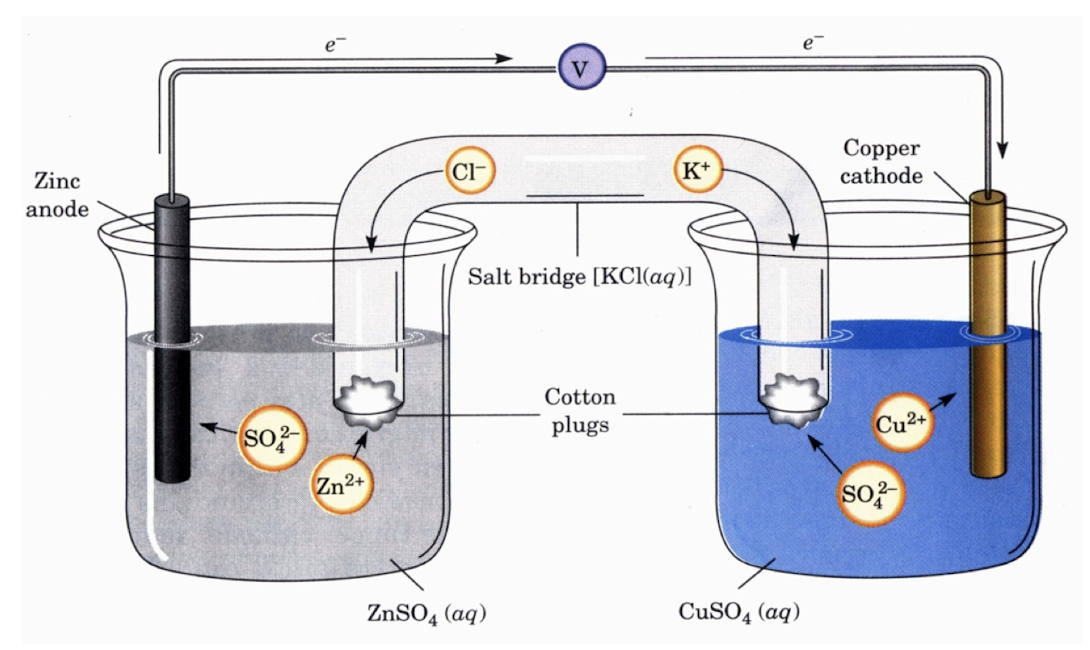
\includegraphics[width=11cm,height=8cm]{battery.png}
\end{figure}
盐桥:充满饱和KCl溶液的U型玻璃管
1. 原电池的构造和原理
构成原电池的三个条件:
\begin{enumerate}[(1)]
\item 必须有一个氧化还原反应
\item 装置内外都要构成电的通路
\item 氧化和还原反应要分别在两个电极上进行
\end{enumerate}
2. 电极类型:\\
\begin{table}[h]
\centering
\begin{tabular}{l|c|c}
\toprule
电极类型& 电对 & 电极符号\\
\hline
金属电极& $Zn^{2+}/Zn$   & $Zn^{2+}\vert Zn$\\
气体电极& $O_{2}/H_{2}O$ & $H^{+}, H_{2}O\vert O_{2}, Pt/C$\\
氧化还原电极& $Fe^{3+}/Fe^{2}$ & $Fe^{3+}, Fe^{2}\vert Pt/C$\\
金属-难溶盐电极& $Ag_{2}O/Ag$ & $OH^{-}\vert Ag_{2}O, Ag$\\
\bottomrule
\end{tabular}
\caption{电极类型}
\end{table}
电极符号中氧化型与还原型限号次序无严格限制\\
惰性电极Pt/C\\
写电极符号时应包含所有影响电极电势大小的所有物质\\
3. 原电池符号\\
\textcircled{1} 负极在左边,正极在右边,盐桥用”$\Vert$“连接 \\
\textcircled{2} 两相界面用”$\vert$“分开,溶液,气体注明$c,p$\\
\textcircled{3} 纯液体,固体和气体卸载惰性电极一边用”$\vert$“分开。\\

\subsubsection{电极电势}
标准电极电势:$\phi^{\theta}$,取决于金属电对的本质,并与金属离子的浓度和溶液的温度有关。\\
标准状态:活度$1.0mol/L$,分压$100kPa$\\
标准氢电极:规定为0\\
标准电极电势测量\\
\begin{figure}[H]
\centering
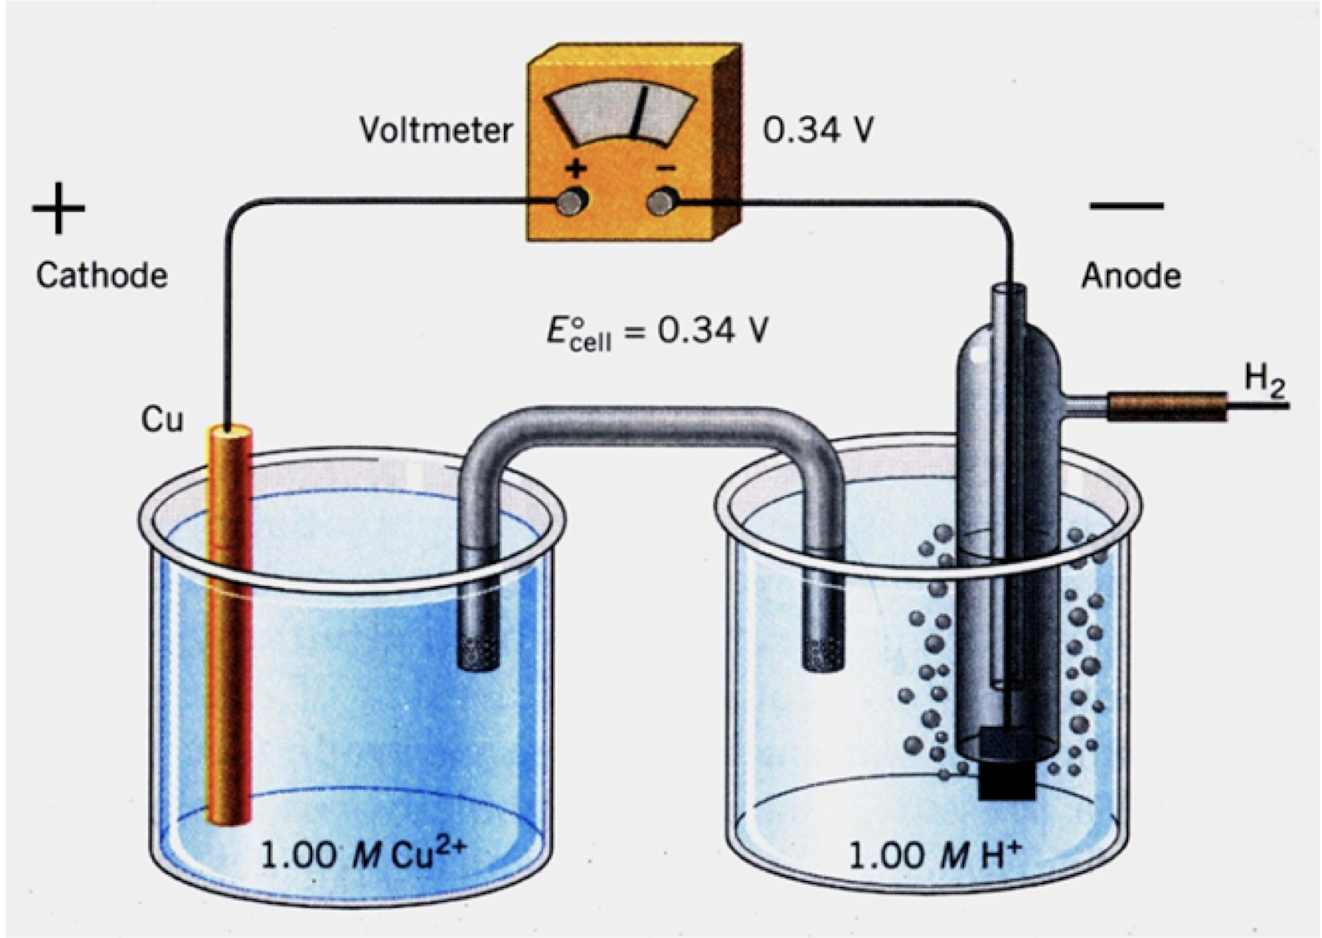
\includegraphics[width=11cm,height=8cm]{E.png}
\caption{电极电势测量}
\end{figure}
计算公式(标准电动势):
\begin{equation}
E^{\theta} = \phi^{\theta}(+) - \phi^{\theta}(-)
\end{equation}
由于氢电极使用条件严格,一般使用参比电极:饱和甘汞电极\\
电极反应:$Hg_{2}Cl_{2} + 2e^{-} \rightleftharpoons 2Hg(I) + 2Cl^{-}$
电极符号:$Hg(I), Hg_{2}Cl_{2}(s)Cl^{-}$\\
$\phi^{\theta} = 0.268V$\\
电极电势与溶液的酸碱性有关\\
注意: \\
a. 反映物质得失电子能力,其大小与电极反应的化学计量数无关(无关于方程式的写法)\\
b. $\phi^{\theta}$为还原电势:待测电极发生还原反应测得的\\
c. 每个$\phi^{\theta}$对应于某一个确定的电对\\
d. $\phi^{\theta}$不具有简单的加和性\\
影响电极电势的主要因素:
\begin{enumerate}[(1)]
\item 温度
\item 浓度
\item 沉淀的生成
\item 配离子的生成
\end{enumerate}
\subsubsection{能斯特方程}
\begin{equation}
\centering
\phi = \phi^{\theta} - \frac{RT}{zF}\ln\frac{a(Red)}{a(Ox)} = \phi^{\theta} - \frac{2.303RT}{zF}\lg\frac{a(Red)}{a(Ox)}
\end{equation}
298K时:
\[
\phi = \phi^{\theta} - \frac{0.0592V}{z}\lg\frac{a(Red)}{a(Ox)}
\]
$z$为转移的电子数目\\
酸性越强,氧化型越强\\
生成沉淀或配离子总结\\
a. 还原型生成配离子或沉淀,还原型浓度减小,$\phi \uparrow$\\
b. 氧化型生成配离子或沉淀,氧化型浓度减小,$\phi \downarrow$\\
\subsection{电极电势的应用}
\subsubsection{计算原电池的电动势}
$\phi^{\theta}$大的做正极,小的做负极。\\
\[
E = \phi(+) - \phi(-)
\]
\subsubsection{判断氧化还原反应进行的方向}
原电池反应中:\\
$E^{\theta}>0.2$,反应向正方向自发进行\\
$E^{\theta}<-0.2$,反应向逆方向自发进行\\
$-0.2<E^{\theta}<0.2$,受到浓度的影响\\
对角线规则
\subsubsection{判断氧化还原反应进行的次序}
\subsubsection{求平衡常数和溶度积常数}
\subsubsection{判断氧化还原反应进行的程度}
\begin{equation}
\lg K^{\theta} = \frac{zE^{\theta}}{0.0592V}
\end{equation}
\subsection{元素电势图及其应用}
具有多种氧化态的远足可以形成多对氧化还原电对,表示元素各氧化碳之间标准电极电势关系的图。\\
{\bf 表示方法}\\
(1) 按照氧化态高到低排列。\\
(2) 两物种之间用横线“——”相连,线上方是标准电极电势,下方是得失电子数。\\
\[
A\stackrel{\phi_1}{——}B\stackrel{\phi_2}{——}C
\]
{\bf 判断歧化反应发生}\\
如果$\phi_{\text{右}}^{\theta}>\phi_{\text{左}}^{\theta}$,发生歧化反应,反之发生反歧化反应。\\
{\bf 计算未知标准电极电势}
\[
\phi^{\theta} = \frac{z_1 \phi^{\theta}_1 + z_2 \phi^{\theta}_2 + z_3 \phi^{\theta}_3 \cdots}{z_1 + z_2 +z_3 \cdots}
\]
\newpage
\section{原子结构}
\subsection{微观粒子的波粒二象性}
\subsubsection{氢光谱与波尔理论}
Balmer经验公式
\[
\lambda  = B(\displaystyle{\frac{n^2}{n^2 - 4}})\qquad B = 364.56nm
\]
Rydberg经验公式
\[
\nu = R(\frac{1}{n_1^2} - \frac{1}{n_2^2})
\]
{\bf 普朗克的量子理论}\\
微观世界中,能量是不连续的,只能以某一最小单位的整数倍变化,称为量子。\\
爱因斯坦提出光子学说\\
提出光具有波粒二象性,$E = h\nu$\\
{\bf 波尔的原子结构理论}\\
(1) 固定轨道理论。原子模型:和外电子围绕确定半径的轨道运动,不吸收和放出能量。最低能量状态是基态,其余为激发态。和外电子只能在某些固定的轨道上运动,这些电子的角动量必须是$h/2\pi$的整数倍。\\
(2) 轨道能量量子化的概念。一定轨道中运动的电子有一定的能量,称为\emph{定态},能量最低的称为\emph{基态},其余称为\emph{激发态}。\\
(3) 能量的吸收和释放。从一个定态到另一个定态要吸收或释放能量。氢原子核外电子通常处于基态,从外部吸收足够的能量才能被激发。从较高能级跃迁到较低能级时,以光子的形式释放能量。\\
局限性:
\begin{enumerate}[a.]
\item 建立在经典物理的基础上,不能解释精细结构、多电子原子光谱、谱线在磁场中的分裂、谱线强度
\item 微观粒子的特殊性不能用经典力学进行解释
\end{enumerate}
\subsubsection{微观粒子的波粒二象性}
1. 光的波粒二象性
\begin{align*}
E = h\nu \\
P = \frac{E}{c} = \frac{h}{\nu}
\end{align*}
2. 电子的波粒二象性\\
大胆预言一切实物粒子都具有波粒二象性。\\
德布罗意关系式
\[
\lambda  = \frac{h}{P} = \frac{h}{mv}
\]
只有在波长远大于粒子时才会表现出波动性。\\
结论:微观粒子不具有波粒二象性,所以不能使用经典力学描述围观粒子的运动,要用量子力学方法。
\subsubsection{测不准原理}
海森堡测不准原理:人们不可能同时准确测定微观粒子的空间位置和动量。
\[
\Delta x\cdot \Delta P_x \geq \frac{h}{2\pi} \approx h
\]
\[
\Delta x\cdot \Delta v \geq \frac{h}{2\pi m}
\]
$\Delta x$表示粒子位置在x方向的不确定值\\
$\Delta P_x$表示粒子动量在x方向的不确定值\\
$\Delta v$表示粒子在运动速度的不确定值\\
几率波:空间任意一点上的波的强度(振幅绝对值的平方)和粒子出现的几率成正比。\\
\begin{table}[h]
\centering
\begin{tabular}{cc}
\toprule
宏观物体&微观粒子\\
\hline
确定的坐标和动量&坐标和动量不能同时确定\\
有连续可测的运动轨道&无运动轨道只能研究概率分布\\
能量任意且连续&能量量子化\\
\bottomrule
\end{tabular}
\caption{宏观粒子与微观粒子对比}
\end{table}
\subsubsection{波函数与薛定谔方程}
1. 波函数\\
微观粒子无法描述运动轨道\\
具有波动性的粒子运动要用波函数表示\\
与$x, y, z$有关\\
2. Schrodinger equation\\
微观粒子在某范围内出现与其环境相关,如$E,V,m$\\\\
\begin{equation}
(\frac{\partial^2\psi}{\partial x^2}+\frac{\partial^2\psi}{\partial y^2}+\frac{\partial^2\psi}{\partial z^2}) + \frac{8\pi^2m}{h^2}(E-V)\psi = 0
\end{equation}
{\fangsong a. 对于质量为m,势能为V的势场中运动的微粒(电子)来说,该方程的每一个合理的$\psi$都代表该粒子的某一个稳定状态。\\
b. $\psi$对应的能量值就是能级\\
c. 方程的解以$\psi(r,\theta,\phi)$表示\\}\\
$n,m,l$为三个量子数,每一个量子数的取值都对应一个合理的解,也就是对应于一个波函数$\psi$。\\
3. 波函数与原子轨道\\
波函数与原子轨道的对应关系:\\
$\psi(1,0,0)$: $1s$轨道; $\psi(2,0,0)$: $2s$轨道;\\
$\psi(1,0,0)$: $2p_z$轨道;\\
这里的原子轨道只是原子运动的一个函数。\\
每一种原子轨道都有与之对应的能量E。\\
\[
\text{波函数} = \text{波函数的合理解} = \text{原子轨道} \cdots\cdots\text{重要}
\]
\subsubsection{波函数和电子云图形}
1. 波函数的角度分布图——原子轨道角度分布
\begin{align*}
\psi_{n,l,m}(r,\theta,\phi) = R_{n,l}(r) \cdot Y_{l,m}(\theta,\phi)
\end{align*}
2. 电子云\\
$\psi^2$表示电子在体积空间内出现的几率,也就是几率密度,形象的表示为电子云。\\
可以用$Y^2$代替$Y$绘制电子云的角度分布图。

波函数的径向部分$R(r)$本身没有意义,但是$r^2R^2$表示电子在离核半径$r$的薄球壳出现的概率。从\figurename{3}可以看出电子按照层分布。

\begin{figure}[H]
\centering
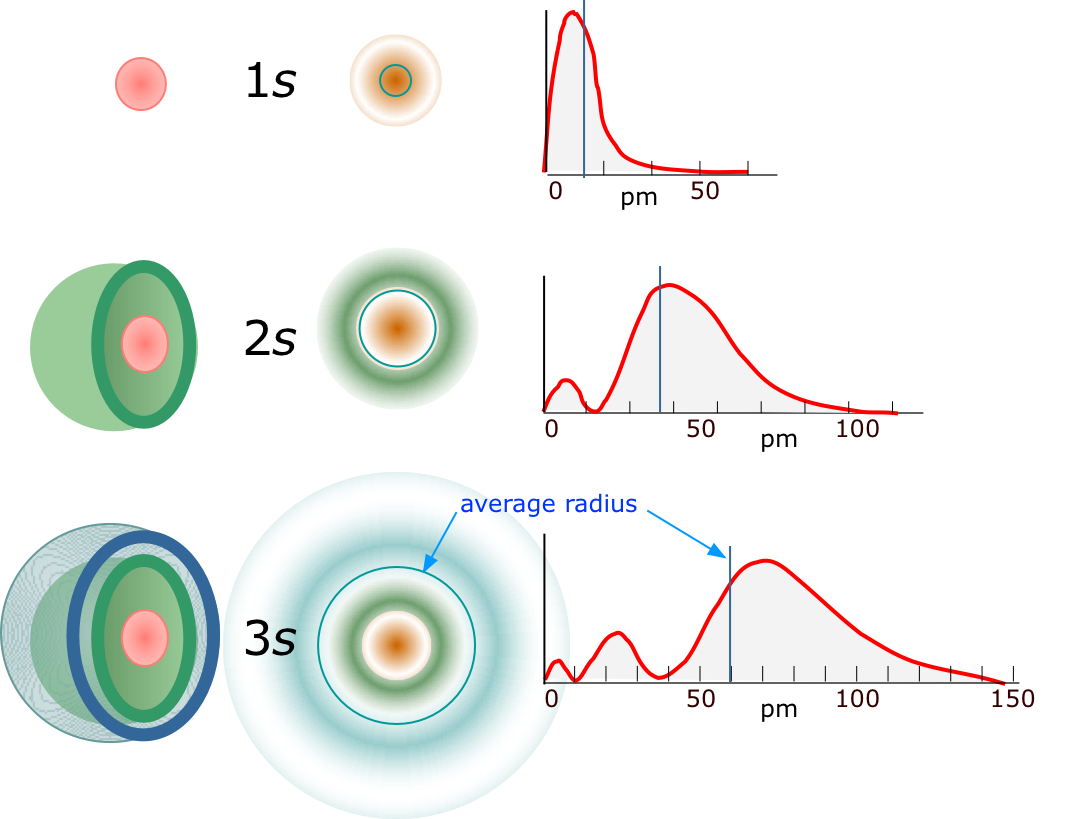
\includegraphics[width=11cm,height=8cm]{s-orb_shells.png}
\caption{关于离核半径}
\end{figure}
\subsubsection{四个量子数}
电子在核外的运动不是任意的,而是只能取一定的运动状态,一般四个量子数才能确定一个电子的运动状态。\\
{\bf 1. 主量子数}\\
表示原子中电子出现概率最大的区域离原子核的远近,是决定电子能级的主要量子数。\\
n只能取正整数\\
每一个n代表一个电子层\\
用大写字母K,L,M,N,……表示电子层\\
对于单电子体系,电子能量唯一决定为n,其他多电子体系还取决于角量子数l。\\
{\bf 2. 角量子数}\\
决定规带角动量,形象的看为决定轨道形状的量子数。\\
l只能取0-(n-1)的正整数。\\
一个l对应一个电子亚层。
\begin{table}[H]
\centering
\begin{tabular}{ccccc}
电子亚层&s,&p,&d,&f……\\
角量子数&0,&1,&2,&3……

\end{tabular}
\end{table}
能量比较:\\
{\centering
n值越大,能量越高;
n值相同,l越大,能量越高}\\
{\bf 3. 磁量子数}\\
同一亚层的几条轨道对原子核的取向不同\\
m的范围$-l \to 0  \to l$的正整数,如p亚层有三种取向,也就是三种轨道。\\
m决定电子云在空间的伸展方向$(2l+1)$个。\\
\begin{figure}[H]
\centering
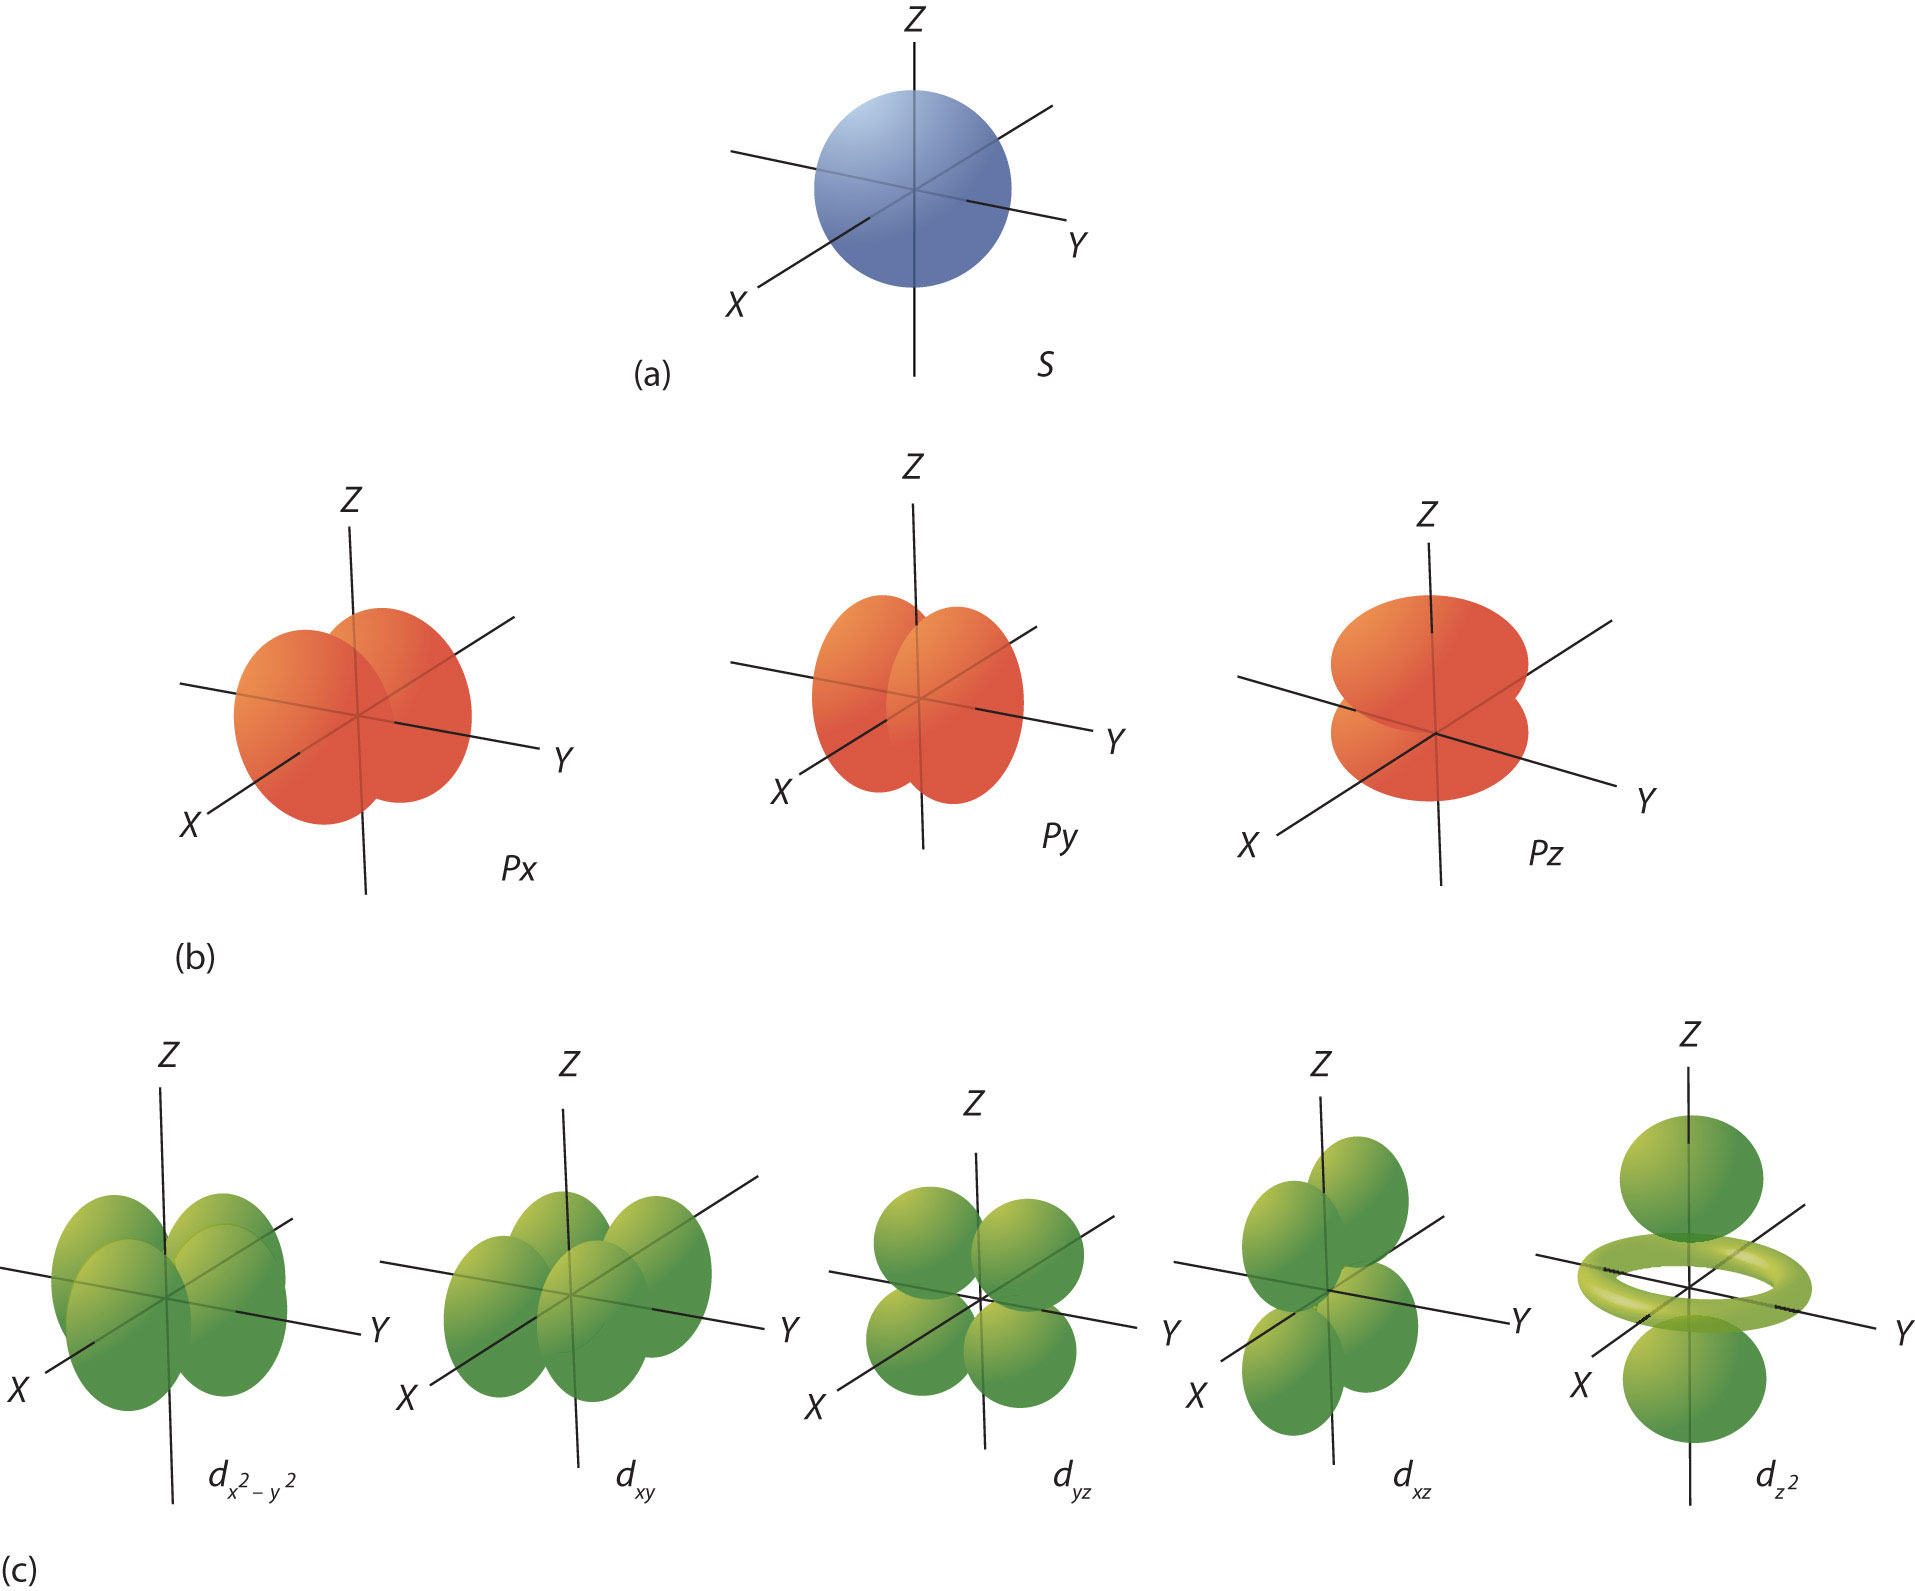
\includegraphics[width=13cm,height=10cm]{Electron Orbitals.png}
\caption{几种分布模式}
\end{figure}
{\bf 4. 自旋量子数$m_s$}\\
$m_s$的取值为$\displaystyle \pm \frac{1}{2}$\\
表示两种自旋方向不同的电子。\\
\begin{figure}[H]
\centering
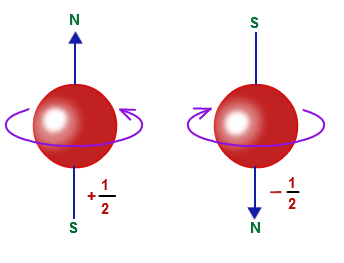
\includegraphics[width=5cm,height=4cm]{spin-quantum-number.png}
\end{figure}
{\bf 小结}
\begin{itemize}
\item 原子中电子运动状态可以用$n,l,m,m_s$四个量子数来描述。
\item 每个电子层中,由于原子轨道形状不同,可有不同分层。
\item 原子轨道在空间伸展方向不同,每一个亚层中可有几个不同方向的原子轨道。
\item 每一个原子轨道可有两个电子处于自旋方向不同的状态。
\item 四个量子数确定电子在核外的运动状态。
\end{itemize}

\subsection{多电子核外电子的运动状态}
\subsubsection{屏蔽效应和钻穿效应}
\emph{多电子原子}:含有两个以上电子的原子,每个电子受到原子核的吸引,同时受到其他电子的排斥。\\
\emph{屏蔽效应}:多电子原子的一个电子受到核的引力和其他两个电子的排斥作用。核外其余电子部分抵消核电荷对于指定电子吸引力的作用。\\
\emph{中心力场模型}:多电子原子中其余电子对指定的某电子的排斥作用近似看做屏蔽了一部分核电荷的吸引力。
\[
Z^* = Z -\sigma
\]
$\sigma$:屏蔽常数\\
$Z^*$:有效核电荷数\\
{\bf 斯莱特(Slater)规则}(\figurename{4})\\
\begin{figure}[H]
\centering
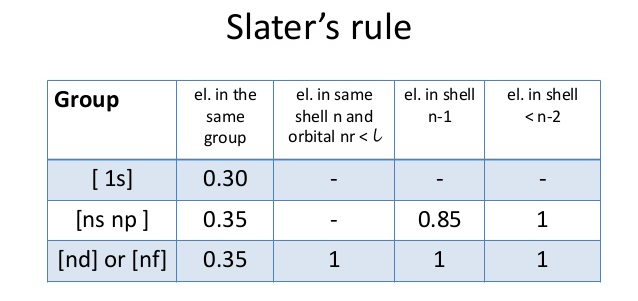
\includegraphics[width=11cm,height=6cm]{slater.png}
\caption{Slater’s Rule}
\end{figure}
对电子分组:将所有的$s$电子与$p$电子分在一起\\
$$(1s)(2s,2p)(3s,3p)(4s,4p)(4d)\cdots$$\\
1) 外层电子对内层无屏蔽\\
2) 组内电子时间有屏蔽($1s$电子$\sigma = 0.3$其余$\sigma = 0.35$)\\
3) 被屏蔽的电子为$ns,np$时,(n-1)层电子$\sigma = 0.85$,(n-2)以及更低$\sigma = 1.00$\\
4) 被屏蔽电子为$nd,nf$时,内侧所有电子$\sigma = 1.00$\\
{\kaishu \small 例:\\
对于钠原子,其$2s$中的一个电子受到的有效核电荷数计算为:
\[
Z^* = 11 - 0.35\times7- 0.85\times2 = 6.85
\]}
{\bf 屏蔽效应对于钾原子电子排布的解释\\}
考虑钾原子的电子排布:\\
(1) $1s^2 2s^2 2p^6 3s^2 3p^6 3d^2  \quad Z = 1.00$\\
(2) $1s^2 2s^2 2p^6 3s^2 3p^6 4s^2  \quad Z = 2.20$\\
{\bf 多电子原子核外电子的钻穿效应}
多电子原子中,某个电子被屏蔽多少与其他电子的数目有关,也与其本身所处的状态有关,如果一个电子在原子核附近出现的几率大,可以避免屏蔽作用,所以其能量更低。\\
这种钻到原子核附近回避其他电子的现象叫做\emph{钻穿效应}\\
径向分布函数的峰值数 = n-l\\
\begin{figure}[H]
\centering
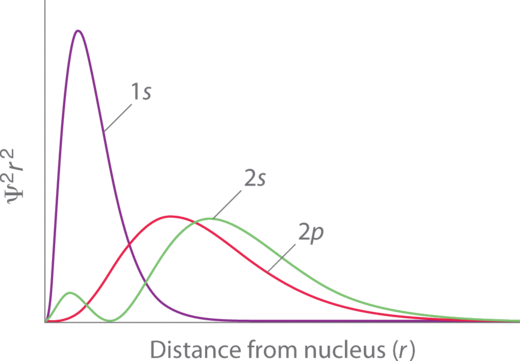
\includegraphics[width = 11cm, height = 8cm]{penetration.png}
\caption{分布函数峰值示意图}
\end{figure}
\subsubsection{原子核外电子排布}
{\bf 泡利不相容原理}\\
在同一个原子钟,不可能存在四个量子数都相同的电子。\\
每个电子层中原子轨道的总数为$n^2$个,所以每个电子层中最多容纳$2n^2$个电子。\\
{\bf 能量最低原理}\\
电子在核外排列尽量分布在低能级轨道上,使整个原子系统能量最低。\\
徐光宪提出使用$n+0.7l$近似计算电子能量高低。\\
\begin{figure}[H]
\centering
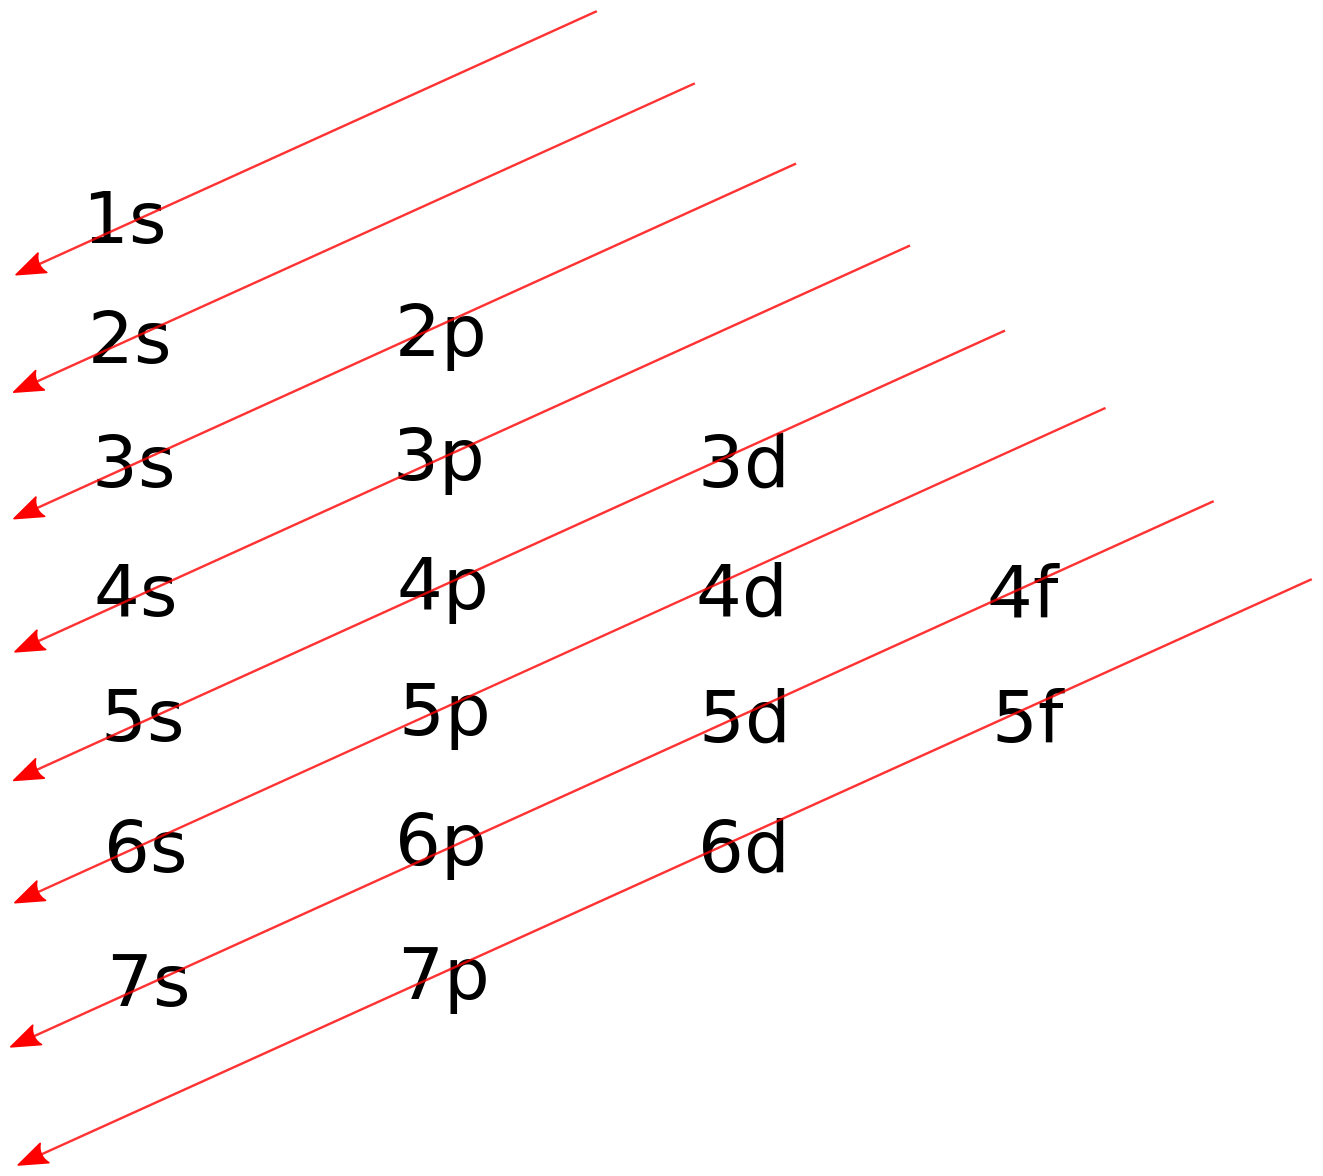
\includegraphics[width = 8cm, height = 7cm]{energy level diagram.png}
\caption{交错原理}
\end{figure}
电子能量大小:\\
当$n$相同,$l$不同,$l$较大的能量较高。\\
当$n$不同,$l$相同,$n$较大的能量较高。\\
当$n,l$均不相同时,使用交错原理进行判断。\\
能量相同的状态称为简并状态。\\
\emph{科顿原子轨道能级图}\\

{\bf 洪特规则}\\
在简并轨道上排布电子时,优先占据不同的轨道且自旋方向相同。\\
特例:等价轨道全充满,半充满或者全空时比较稳定\\
$^{24} Cr\quad 1s^2 2s^2 2p^6 3s^2 3p^6 {\bf 4s^1 3d^5}$\\
在书写时,可以将达成稳定的电子层写成稳定气体的形式:\\
$Fe:[Ar]3d^64s^2$\\
{\bf 电子排布的例外}:\\
核外电子排布三规则只是一般规则,但是随着原子序数的增加,核外电子数目的增多以及原子中电子间相互作用的复杂化,出现了一些例外。\\
离子的电子排布:失电子顺序由外层到内层逐层失去。
\subsection{原子结构和元素周期表}
\subsubsection{核外电子排布和周期表的关系}
1. 原子的电子层的结构\\
\emph{元素周期律}:元素性质随核电荷数递增而呈现周期性变化。\\
\begin{figure}[H]
\centering
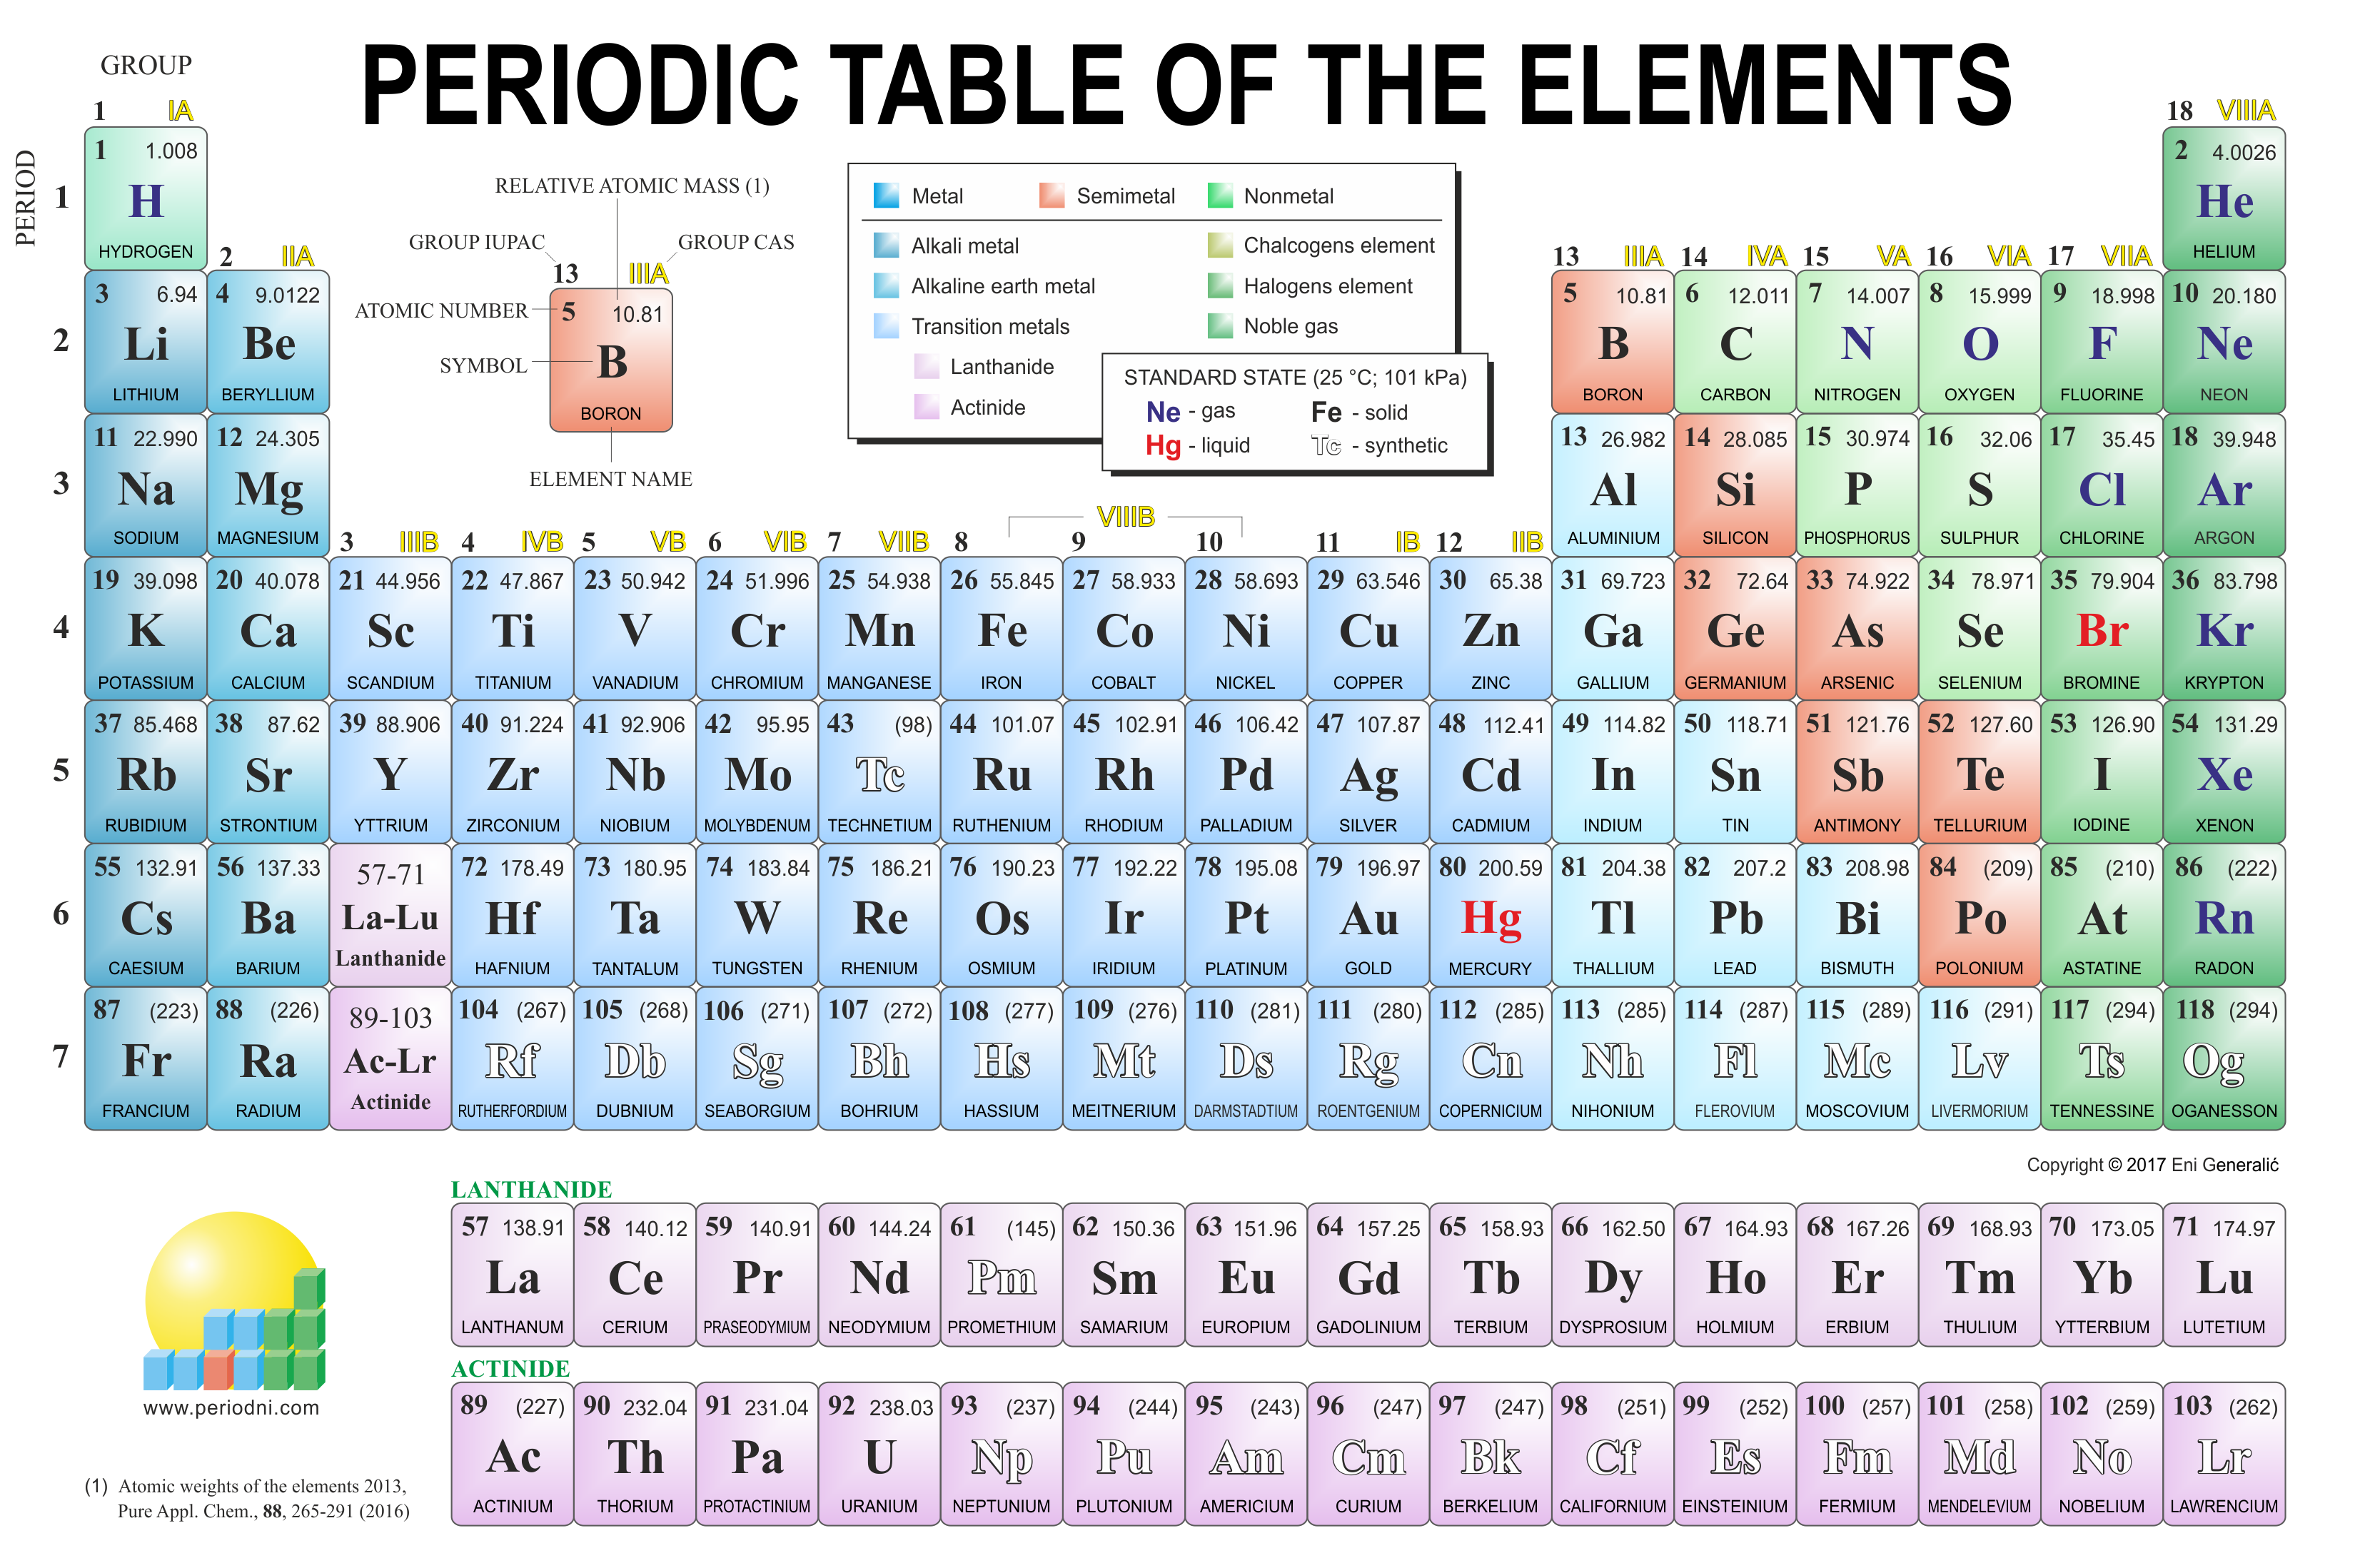
\includegraphics[width = 18cm, height = 12cm]{modern_periodic_table.png}

\end{figure}
2. 周期和族\\
周期数 = 能级组组数 = 电子层层数\\
各周期元素数目 = 个电子层原子轨道所能容纳的电子总数\\
族对应于电子数:
\begin{itemize}
\item 主族元素的族数 = 最外电子层的电子数,最外层s电子+p电子
\item 零族(惰性气体)最外层s电子+p电子=8
\item 副族元素的族数 = 最外层电子数 + 次外层d电子(VIII,IB,IIB)
\item 第八族:最外层电子数+次外层d电子数 = 8,9,10
\end{itemize}
3. 元素分区
\begin{table}[H]
\centering
\begin{tabular}{ll}
\toprule
\multicolumn{1}{c}{区} & \multicolumn{1}{c}{价电子构型}\\
\hline
s区: & $ns^{1\sim2}$\\
p区: & $ns^2np^{1\sim6}$\\
d区: & $(n-1)d^{1\sim8}ns^2$(少数特例)\\
ds区: & $(n-1)d^{10}ns^{1\sim2}$\\
f区: & $(n-2)f^{1\sim14}ns^2$(少数特例)\\
\bottomrule
\end{tabular}
\end{table}
\subsubsection{原子结构与元素基本性质}
{\bf 1. 原子半径}\\
最外层电子离核距离决定原子的半径\\
共价半径:适用于非金属元素,它们核间距离一半。\\
金属半径:适用于金属元素,相邻原子核间距离一半。\\
van der waals半径:两个原子只靠分子间相互作用力吸引时,其核间距离的一半。(如惰性气体)\\
\emph{原子半径变化规律:}
\begin{enumerate}[1)]
\item 从左到右,原子半径逐渐减少,核电荷增大,零族元素原子半径大幅增加(计算方式不同)。
副族元素下降比主族慢:排布在$d$轨道上,屏蔽效应更强。
\item 同一主族从上到下,原子半径逐渐增大,电子层的增加使原子半径增大。
副族元素增加比主族慢,甚至在出现镧系收缩
\item 镧系收缩:镧系元素的原子半径随原子序数增加逐渐减少。导致第六周期大于第五周期
\end{enumerate}
\begin{figure}[H]
\centering
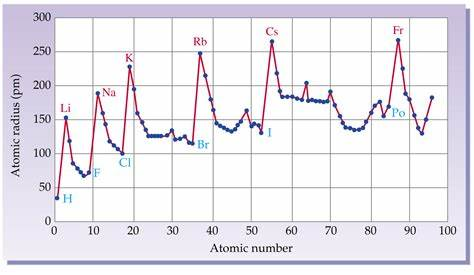
\includegraphics[width=11cm,height=5cm]{atomic radius.jpeg}
\caption{原子半径}
\end{figure}
{\bf 2. 电离能}
基态气体原子失去一个电子成为带一个正电荷的气态离子所需要的能量称为第一电离能,用$I_1$表示。\\
+1价气态正离子失去电子成为+2价气态正离子需要的能量为第二电离能,用$I_2$表示。\\
$I_1$越小,元素越容易失去电子,金属性越强。\\
Remark: 电离能的大小只能衡量气态原子失去电子变为气态离子的难易程度,金属在溶液中发生化学反应形成阳离子的倾向应该根据金属的电极电势来衡量。\\
\emph{电离能变化周期规律}
\begin{enumerate}[1)]
\item 同一周期从左到右增大,主族元素增加明显,过度元素变化不大。
\item 同族元素从上到下减小。
\item 达到全满或半满比较稳定。(如B,Mg,Zn,Cd,Hg,N,P)($I_1(O)<I_1(N)$)
\end{enumerate}
\begin{figure}[H]
\centering
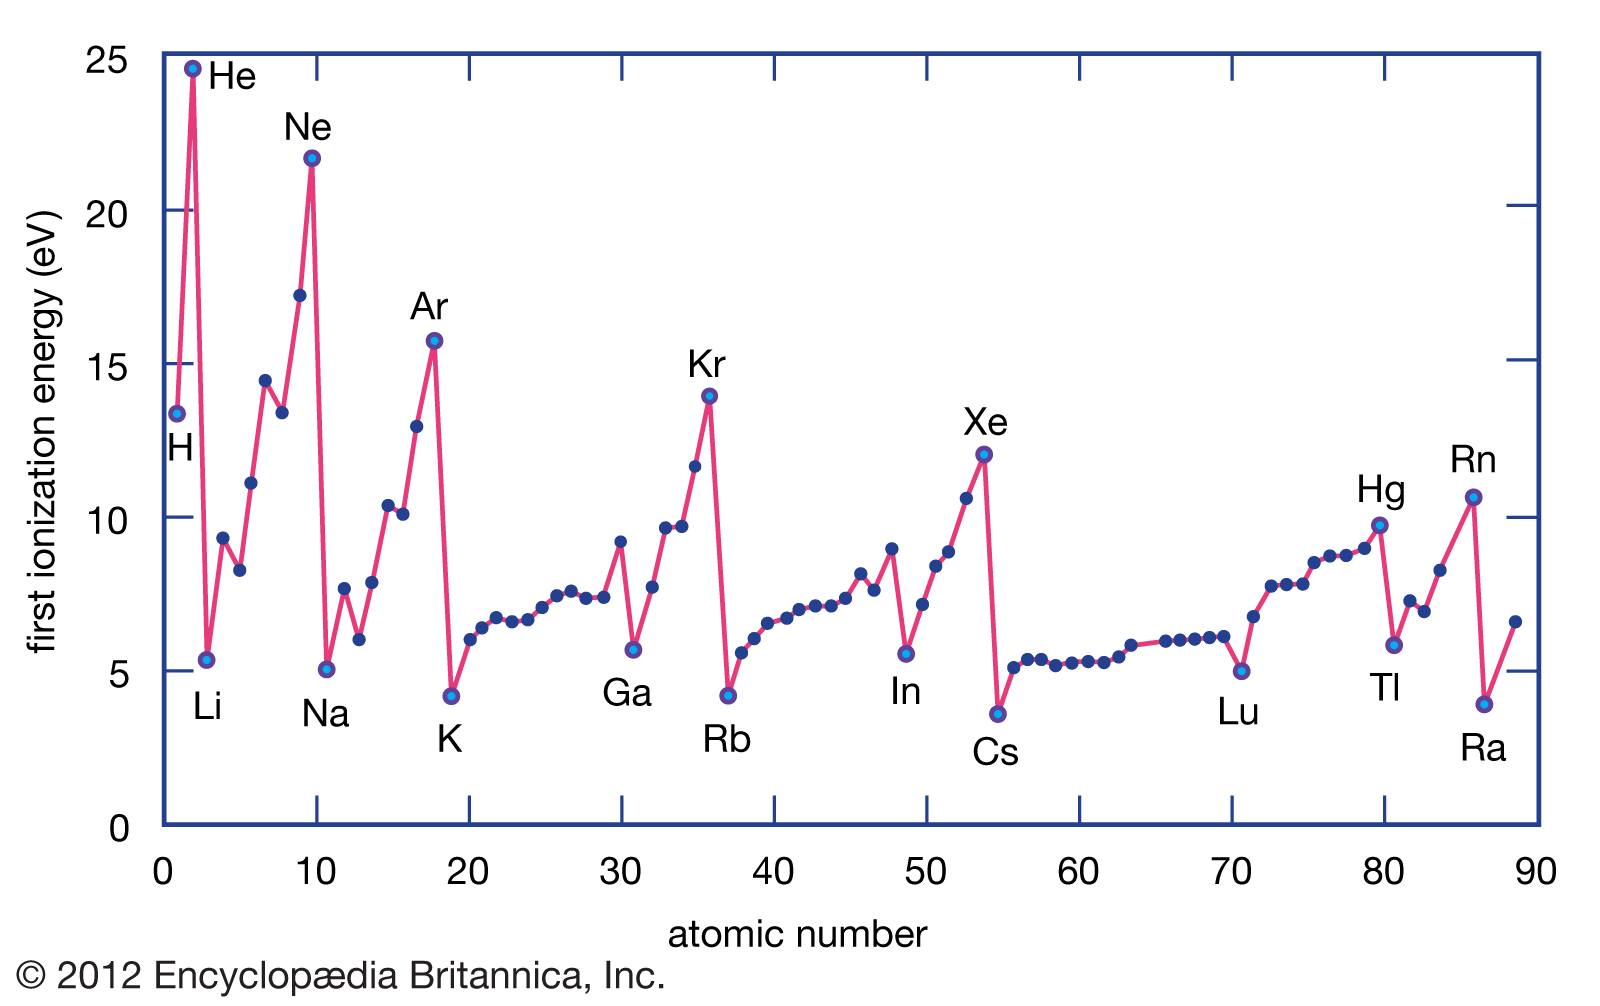
\includegraphics[width=11cm,height=5cm]{ionization-energy-element-atom-electron-energies-nonmetal}
\caption{第一电离能}
\end{figure}
{\bf 3. 电子亲和能(E)}\\
元素的气态原子在基态时获得一个电子成为一价负离子所释放出的能量称为电子亲和能。\\
当负一价离子再获得电子时要克服负电荷之间的排斥力,因袭要吸收能量。放热是正,吸热为负。\\
\emph{电子亲和能一般规律:}
\begin{enumerate}[1)]
\item 元素原子的第一电子亲和能一般都为正值。
\item 只有稀有气体和IIA族原子由于最外层排满,所以为负值。
\item 所有原子的第二亲和能都为负值,由于离子带负电荷。
\item 从左到右逐渐增加,从上到下逐渐减少。
\item 例外:第二周期低于第三周期(第二周期原子半径特别小,电子云密度过高),第二主族低于第一主族(全满全空结构)。
\end{enumerate}
\begin{figure}[H]
\centering
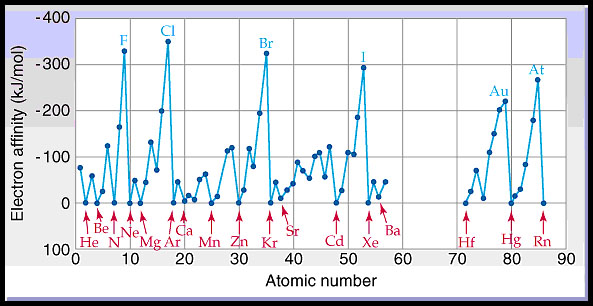
\includegraphics[width=11cm,height=5cm]{electron-affinity.jpg}
\caption{亲和能}
\end{figure}
{\bf 4. 电负性}\\
分子中的原子对成键电子的相对吸引力。无量纲\\
电负性标度:Pauling电负性标度,F的电负性为4.0\\
\emph{电负性变化周期规律:}
\begin{enumerate}[1)]
\item 从左到右递增
\item 从上到下递减
\item 副族元素变化不明显
\end{enumerate}
\begin{figure}[H]
\centering
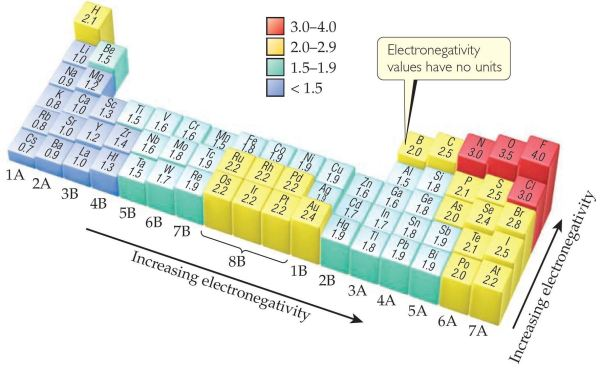
\includegraphics[width = 11cm,height= 7cm]{electronegativity-trends.jpg}
\caption{电负性}
\end{figure}
\begin{figure}[H]
\centering
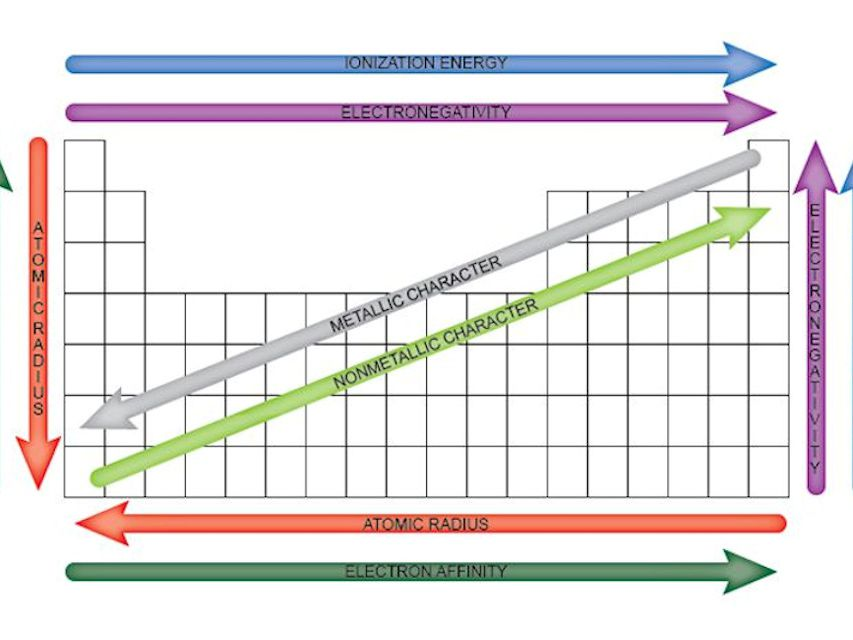
\includegraphics[width = 11cm,height= 7cm]{trend.jpg}
\caption{变化规律总结}
\end{figure}

\newpage
\section{分子结构}
\subsection{离子键}
\subsubsection{离子键理论}
离子键:正负离子之间的静电引力而形成。\\
离子型化合物以离子晶体的形式存在,而不是离子型分子的形式存在。\\
{\bf 离子键的特点}\\
本质是静电相互作用\\
离子性与电负性相关,差值越大,离子型越强。\\
没有方向性\\
没有饱和性:周围的异电荷离子数取决于正负离子的相对大小,还可以吸引远层异电荷离子。\\
离子性物质不存在单个分子:NaCl只代表比例。\\
离子型化合物:离子键组成的化合物\\
离子晶体:由正离子和负离子结合而成的晶体。\\
(1) 质点间作用力是静电作用力。\\
(2) 熔沸点和硬度高。\\
(3) 多数化合物易溶于水。\\
(4) 多数化合物易溶于水。\\
(5) 离子晶体中,每个离子都被若干个异电荷电子所包围,形成一个大分子。\\
\subsubsection{离子的特征}
{\bf 1. 离子半径}\\
\emph{离子半径变化规律}
\begin{enumerate}[1)]
\item 同族元素离子半径由上到下递增
\item 同周期正离子半径随离子电荷增大而减小;负离子随电荷增大而增加。
\[Na^+>Mg^{2+}>Al^{3+}, O^{2-}>F^-\]
\item 对于等电子离子而言,离子半径随着电负性的降低和正电荷的升高而减小
\[ O^{2-}>F^->Na^+>Mg^{2+}>Al^{3+}\]
\item 元素周期表中处于相邻的左上方和右下方对角线上的正离子半径近似相等。
\end{enumerate}
\begin{figure}[H]
\centering
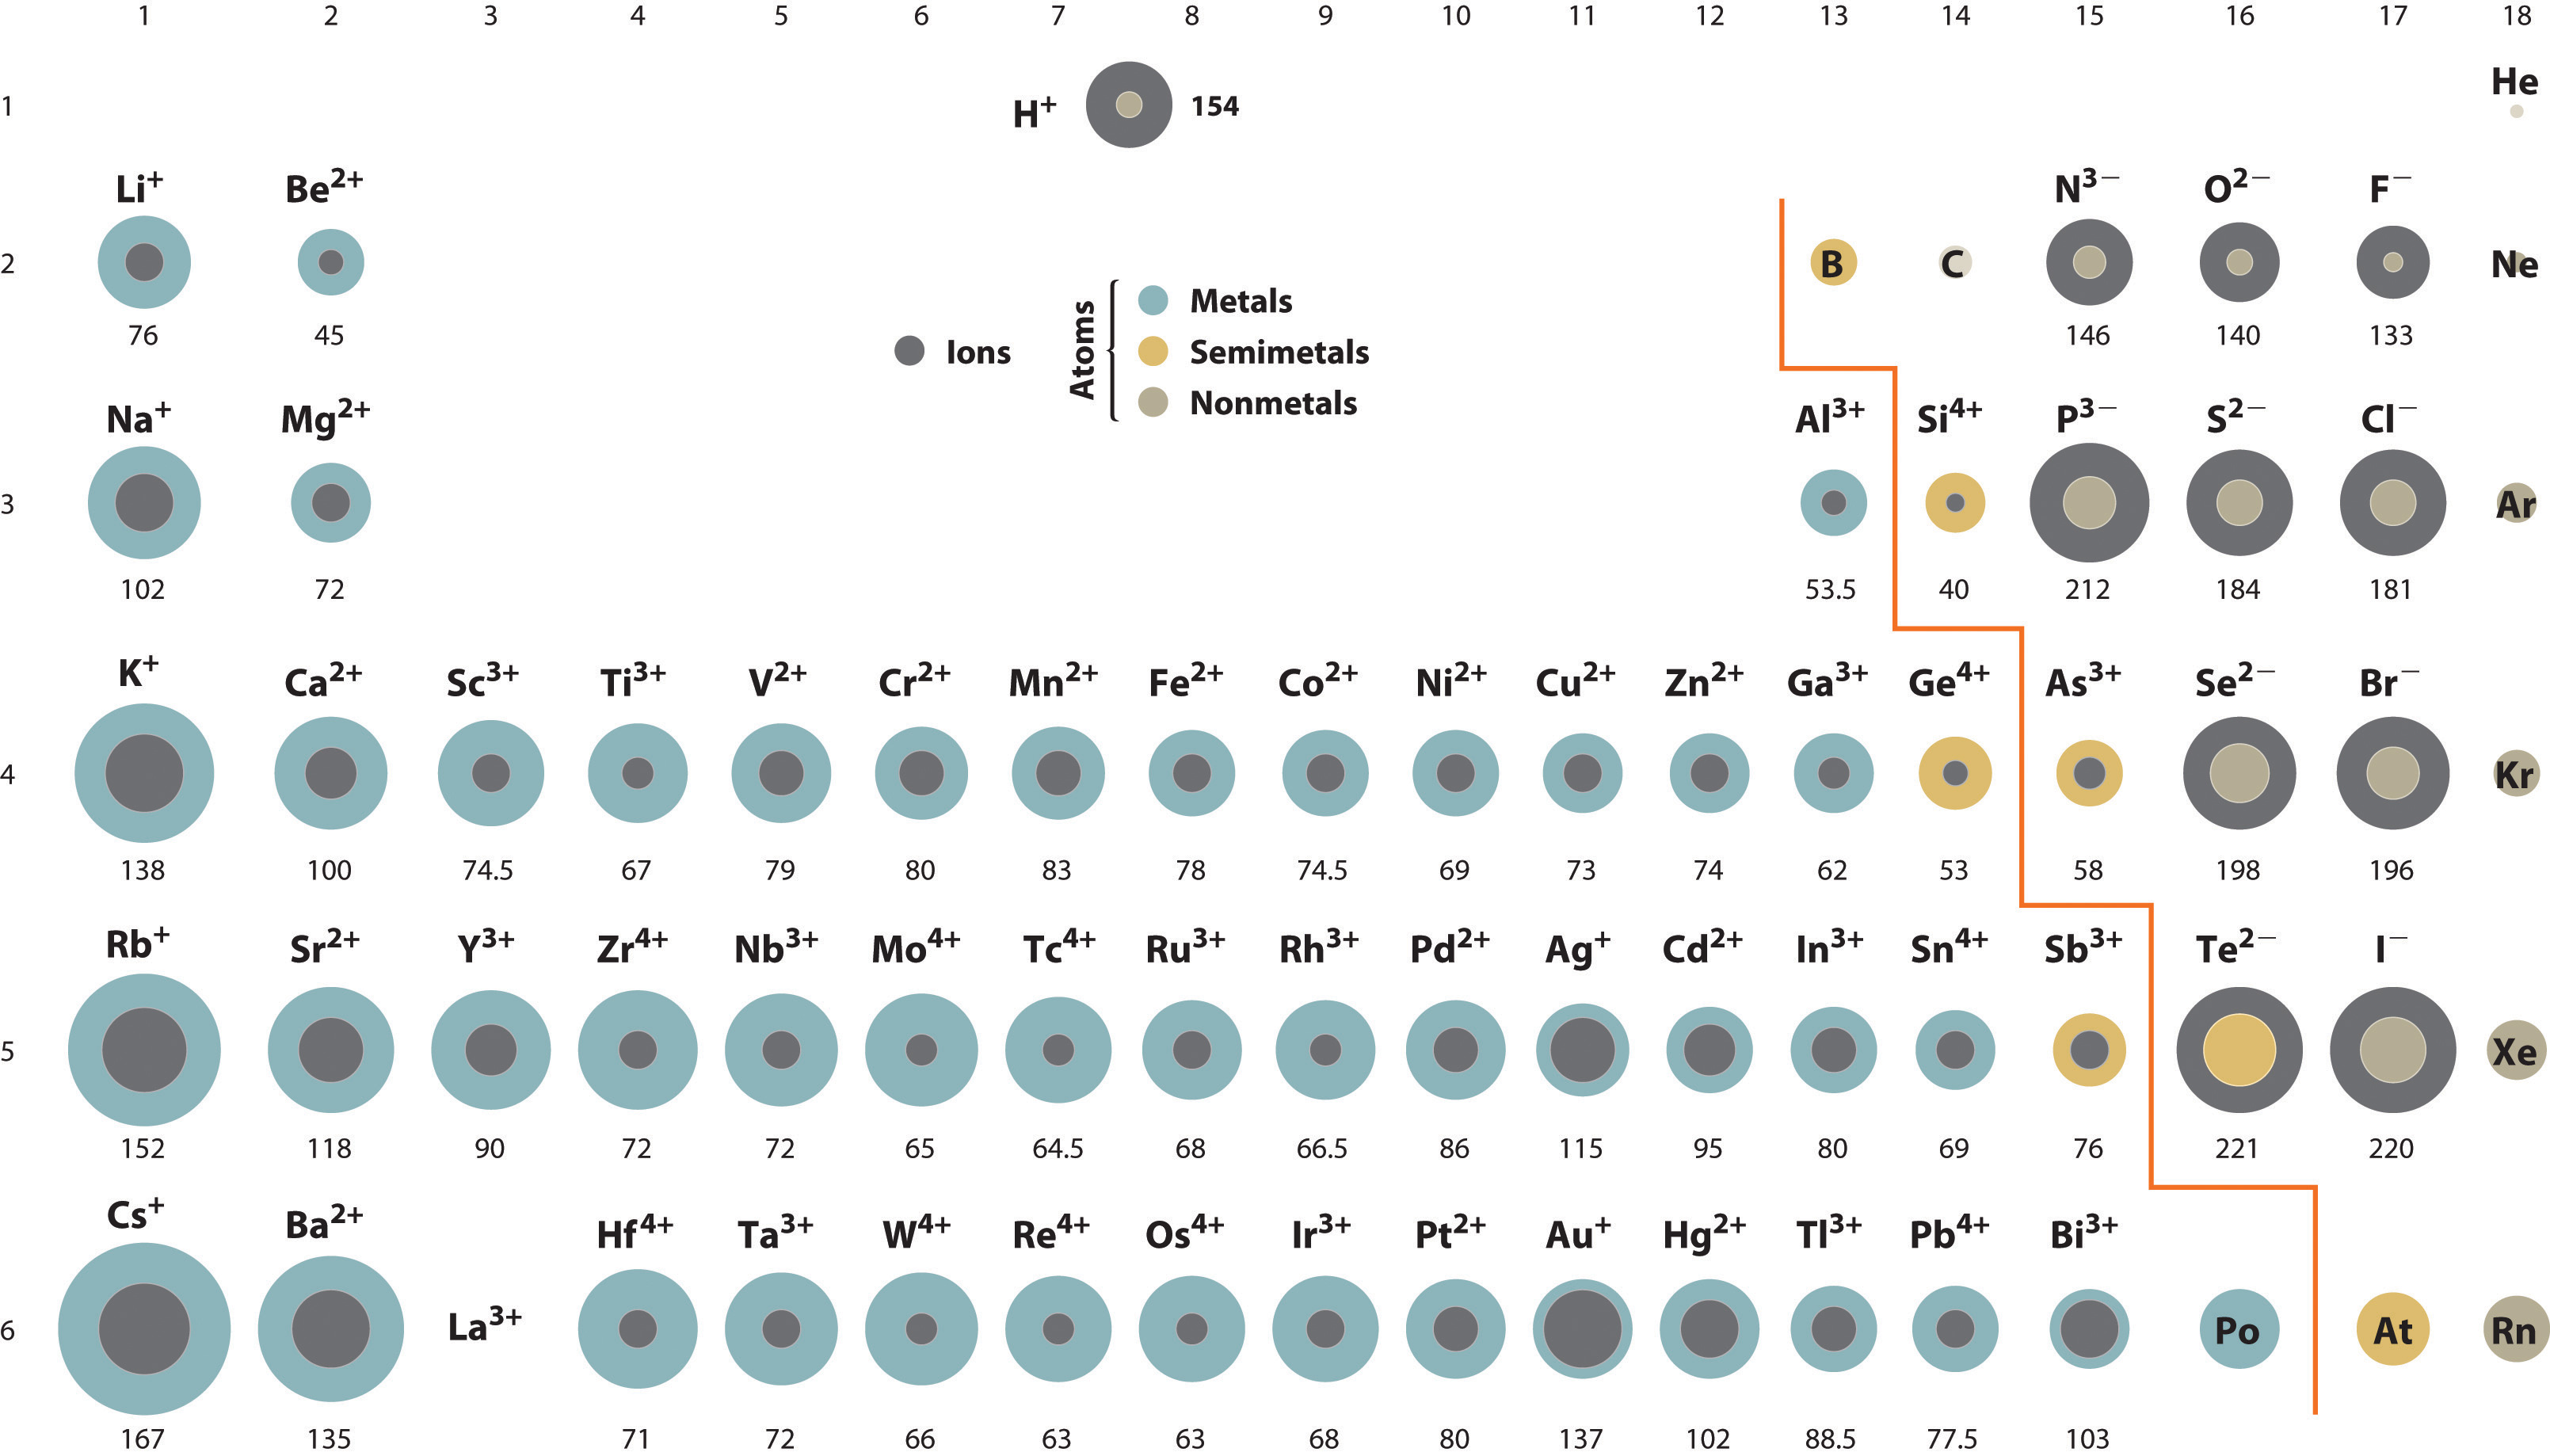
\includegraphics[width=13cm,height=8cm]{ion radius.jpg}
\caption{离子半径}
\end{figure}
离子半径大小对离子化合物性质的影响\\
a. 半径越小,离子键越强,化合物熔沸点越高\\
b. 半径越大,共价性增强,水中溶解度降低\\
判断两种元素之间形成离子键或共价键的方法\\
电负性差值大于1.7倾向于形成离子键,小于1.7倾向于形成共价键\\
Remark: 化合物不存在百分百的离子键,电负性差值大于1.7事实上是离子键成分大于50\%\\
离子半径与配位比的关系(只适用于AB型离子晶体)\\
\[r^+/r^-\]
{\bf 2. 离子电荷}\\
正离子通常只由金属原子形成,其电荷等于中性原子失去电子的数目。(容易达到稀有气体稳定结构或d轨道全充满的结构)\\
通常来讲正离子电荷数不会超过4\\
例外:$NH_4$离子\\
负离子通常只由非金属原子形成,其电荷等于中性原子获得电子的数目\\
{\bf 3. 离子的电子构型}\\
单原子负离子:通常具有稳定的8电子构型$Cl^-,S^{2-}$\\
单原子正离子\\
\subsubsection{晶格能}
定义:气态正离子与气态负离子结合生成1mol离子晶体时所释放的能量。\\
晶格能越大:熔沸点越高,硬度越大,压缩系数和膨胀系数小。

\subsection{共价键和价键理论}
离子键理论无法解释单质分子和电负性相近的原子如何形成化合物。\\
\subsubsection{价键理论}
通过共用电子对使每一个原子达到稳定的稀有气体电子结构\\
Lewis理论的局限性:\\
(1) 不能解释为什么共用使得原子紧密结合\\
(2) 不能解释某些分子的一些性质\\
(3) 有很多例外\\
(4) 不能解释方向性和饱和性\\
现代价键理论:\\
(1) 配对成键:自旋相反的单电子的原子相互接近时,单电子可以配对构成共价键。从而使体系的能量降低\\
(2) 原子轨道最大重叠:重叠较大的电子密度对于两核的吸引力。重叠越大,吸引力越强,越稳定。\\
\subsubsection{共价键的特征}
{\bf 1. 共价键的饱和性}\\
每个原子成键的总数或以单键连接的原子数目是一定的。\\
{\bf 2. 共价键的方向性}\\
原子轨道有一定的方向性。为了满足最大重叠原理。造成了共价键的方向性。\\
对称性原则:对称性相同的部分重叠时,两原子间电子出现的几率才会增加,才可能形成化学键\\
{\bf 3. 共价键的类型}\\
共价键分为两类:$\sigma$键和$\pi$键。\\
(1) $\sigma$键:按照头碰头的方式发生重叠,则键轴是成键原子轨道的对称轴,这种共价键称为$\sigma$键\\
(2) $\pi$键:原子轨道按照肩并肩的方式形成的共价键。$\pi$键的键能较低,稳定性较低,是化学反应的积极参与者。\\
配位共价键:一条充满电子的轨道和一条空轨道形成配位共价键。

\subsection{杂化轨道理论}
\subsubsection{杂化轨道理论的基本要点}
定义:同一原子中能级相近的不同类型的若干原子轨道(波函数)相互作用,改变原有形态,重新组合成一组成键能力更强的新轨道。这种重新组合的过程称为杂化。激发和杂化同时进行。只有在形成分子的过程中才会进行杂化。\\
杂化的特性:\\
杂化只发生在能量相近的一组轨道之间。如ns-np,ns-np-nd,(n-1)d-ns-np。\\
杂化轨道的成键能力大于未杂化轨道。\\
杂化轨道的数目等于参与杂化的轨道的总数。\\
伸展方向与其轨道数和轨道类型有关。\\
\emph{不一定具有未成对电子,可能有空轨道}
\subsubsection{杂化轨道的类型}
\begin{figure}[H]
\centering
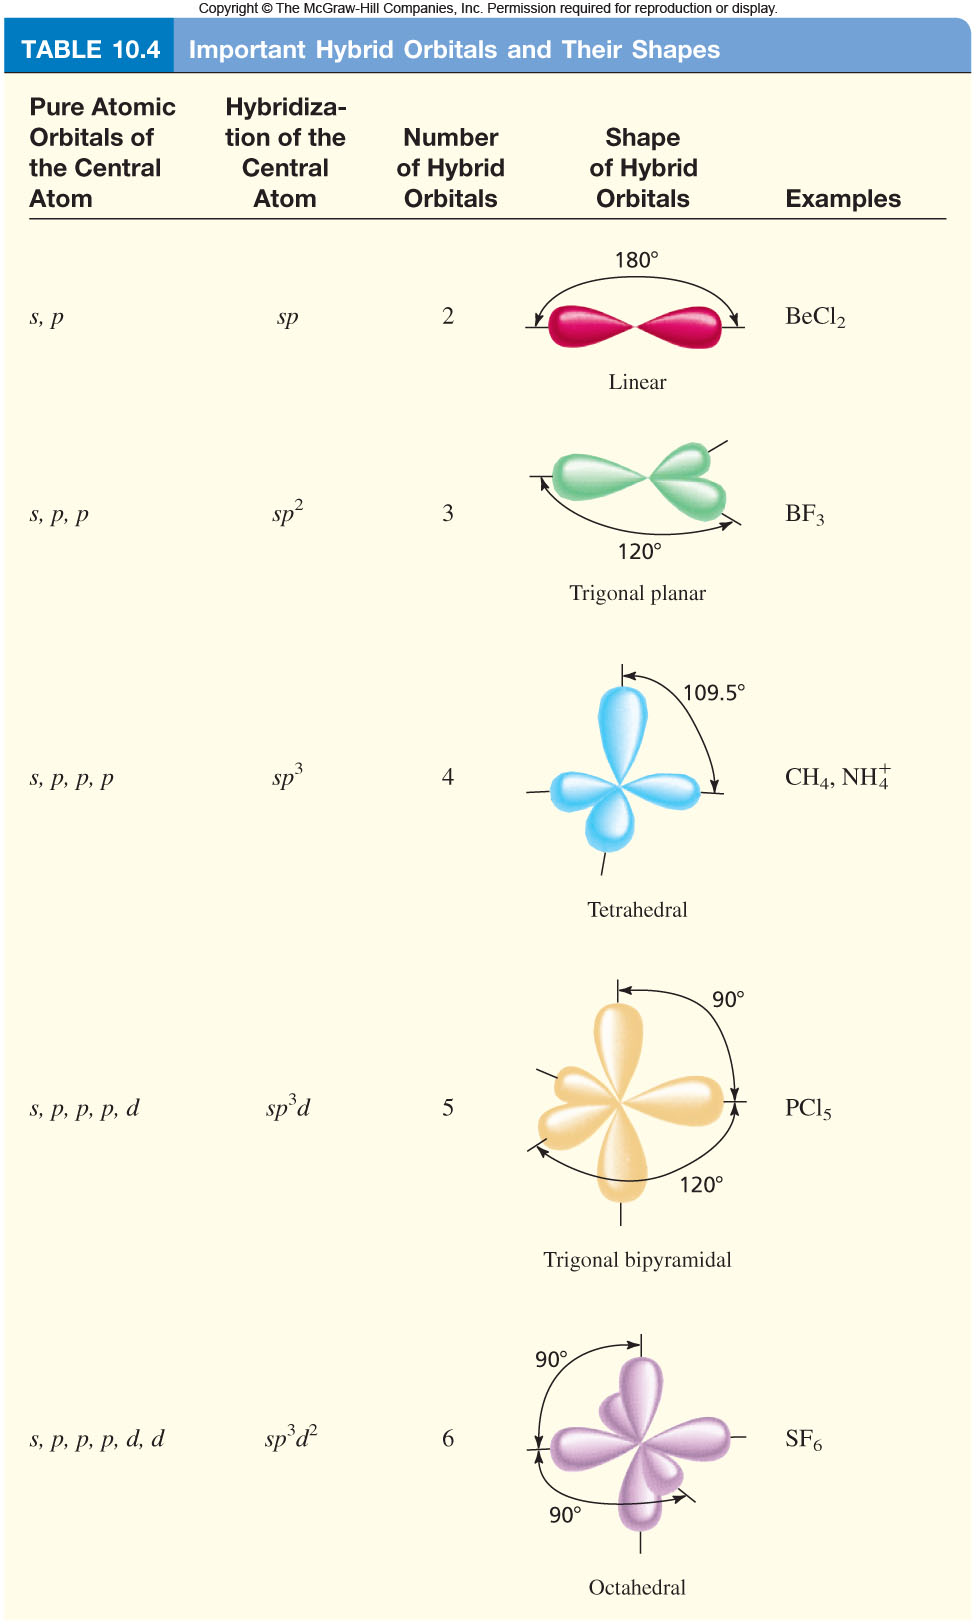
\includegraphics[width=7cm,height=11cm]{Hybrid_Orbitals.jpg}
\caption{杂化轨道示意图}
\end{figure}
$dsp^2$杂化:平面正方形\\
不等性杂化:参与杂化的轨道中存在有孤对电子,杂化后含有的s和p成分不完全相等(孤对电子s成分多,p成分少;成键电子相反),这样的杂化轨道称为不等性杂化轨道。(如氨分子的结构)\\
\begin{figure}[H]
\centering
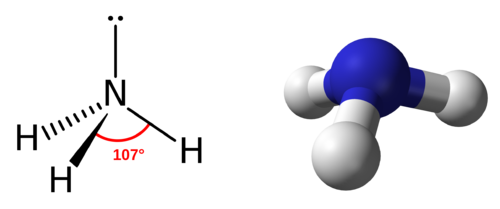
\includegraphics[width=7cm,height=3cm]{ammonia.png}
\caption{氨分子结构}
\end{figure}
\subsection{价层电子对互斥理论(VSEPR)}
分子$AB_n$型分子中,A为中心,B为配体。本节中,A为主族元素的原子;$AB_nL_M$为含有孤对电子的分子。\\
价层电子:A价层内的成键电子对和孤电子对的统称。\\
基本要点:\\
1. 价层电子对数 = (中心原子价电子数 + 配位原子提供电子数 - 离子电荷代数值)/2\\
2. 使孤对电子成$90^{\circ}$的情况尽量少。
\begin{table}[H]
\centering
\begin{tabular}{c|ccccc}
\toprule
电子对数&2&3&4&5&6\\
\hline
电子对排布&直线&平面三角&四面体&三角双锥&八面体\\
\bottomrule
\end{tabular}
\end{table}
\subsection{分子轨道理论}
\subsubsection{分子轨道理论的基本要点}
{\bf 1. 电子在整个分子中运动}\\
{\bf 2. 由原子轨道线性组合而成,分子轨道数目等于参与组合的原子轨道数目}
\begin{align*}
\psi_1 = \psi_{1s} + \psi_{1s}\quad\text{成键轨道,能量降低} \\
\psi_2 = \psi_{1s} - \psi_{1s}\quad\text{反键轨道,能量升高}
\end{align*}
3. 不同的分子轨道能量不同\\
4. 每个分子轨道都有相应的图像,根据组合方式不同分为$\pi$轨道和$\sigma$轨道\\
5. 分子轨道中电子排布遵循原子轨道电子排布三原则
\subsubsection{分子轨道能级图}
相关性:与原子轨道的能量高低、原子轨道之间的相互作用有关。\\
一般来说,原子轨道能量越低,分子轨道能量越低。\\
{\bf 双原子分子轨道能级图}\\
\begin{figure}[H]
\centering
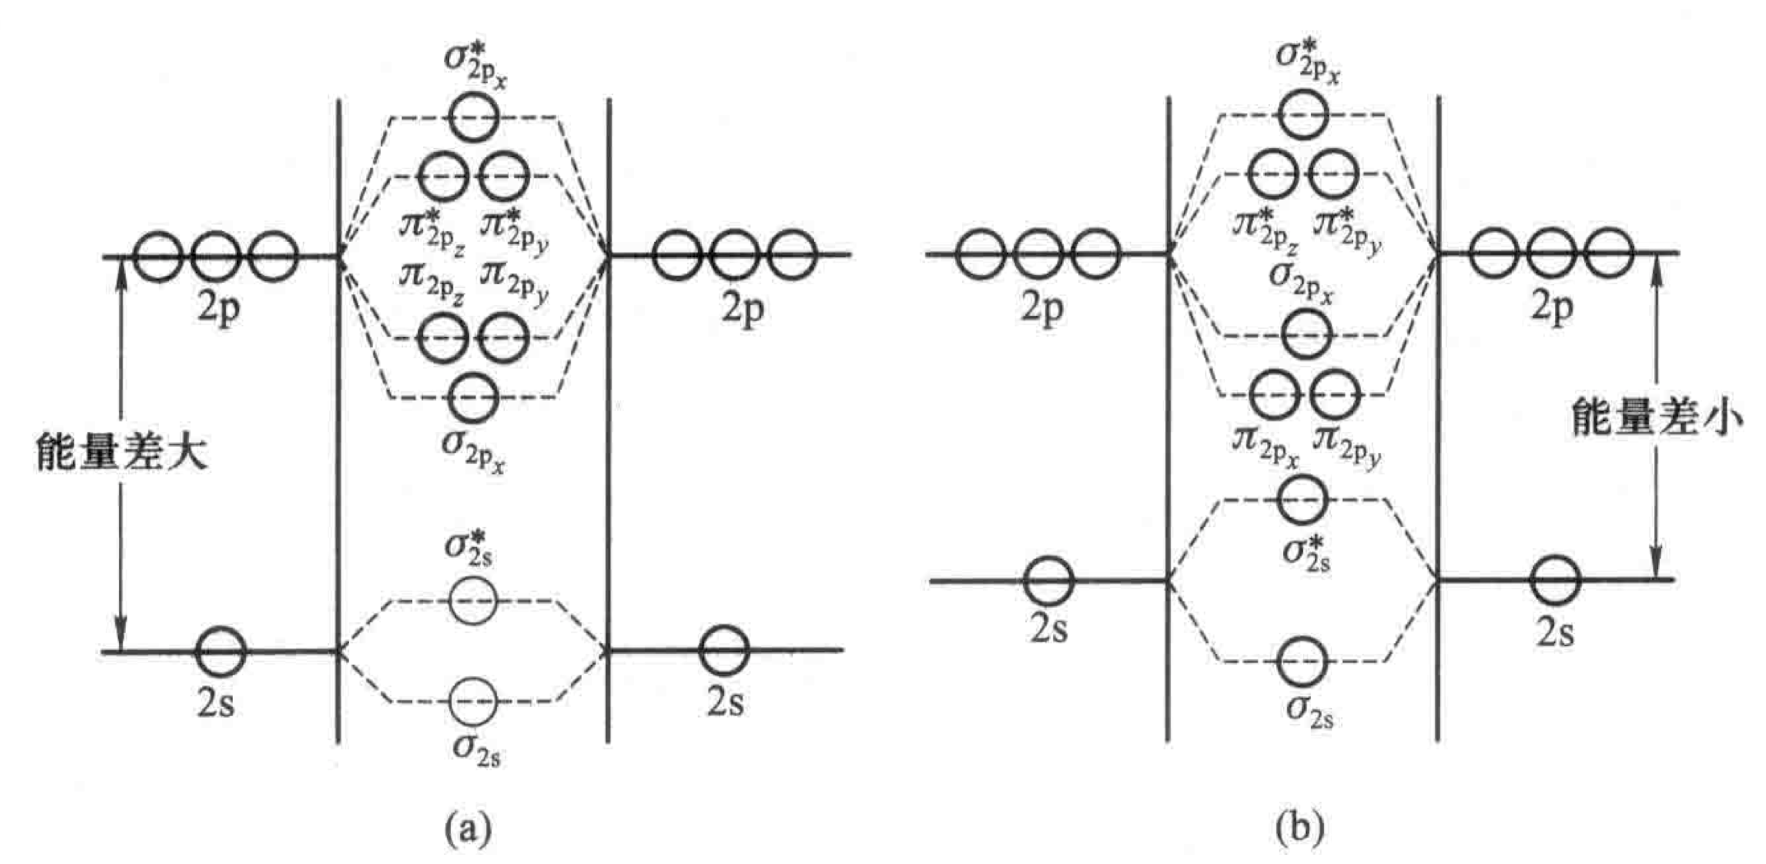
\includegraphics[width = 14cm,height=7cm]{MO.png}
\caption{(a)氧,氟(b)氧,氟之后}
\end{figure}
根据原子轨道排布的三原则依次填充电子\\
键级 = (成键轨道电子数 - 反键轨道电子数)/2\\
\begin{figure}[H]
\centering
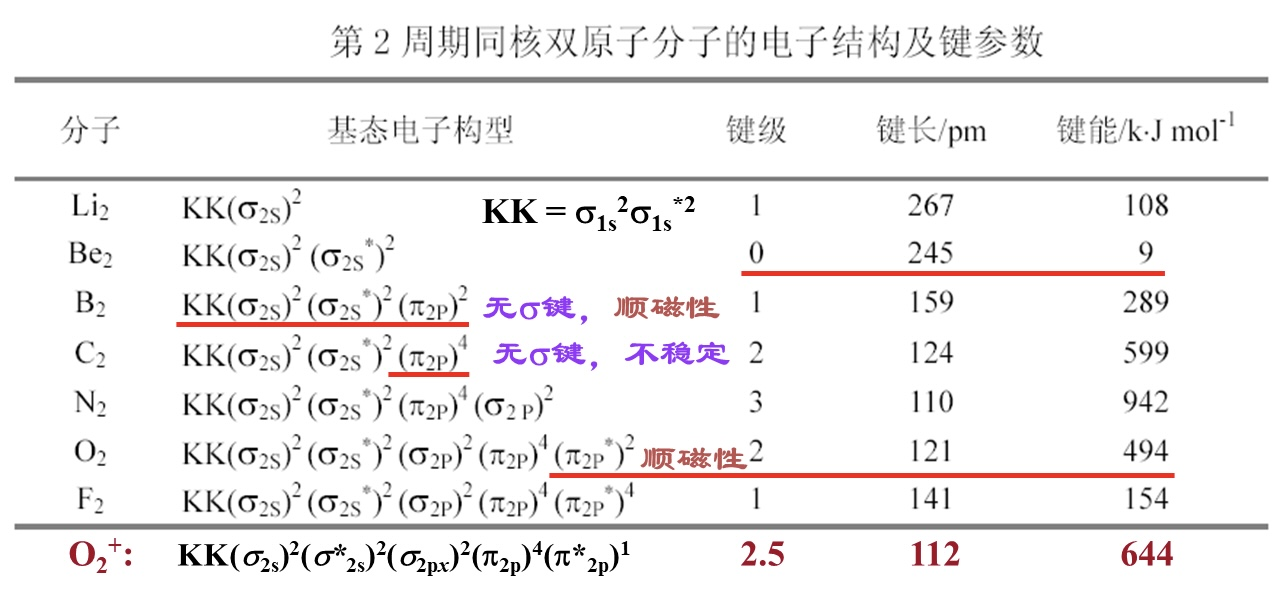
\includegraphics[width=11cm,height=6cm]{MO electron.jpg}
\caption{分子轨道排布}
\end{figure}
等电子体:$CO$和$N_2$都有14个电子,结构、某些性质相似\\
\subsubsection{分子轨道理论的应用}
预测分子或离子的存在\\
{\small \kaishu 预测$H_2^+$是否存在}\\
%氧的分子轨道,解释磁性
氧的顺磁性:分子轨道上有两个单电子
\begin{figure}[H]
\centering
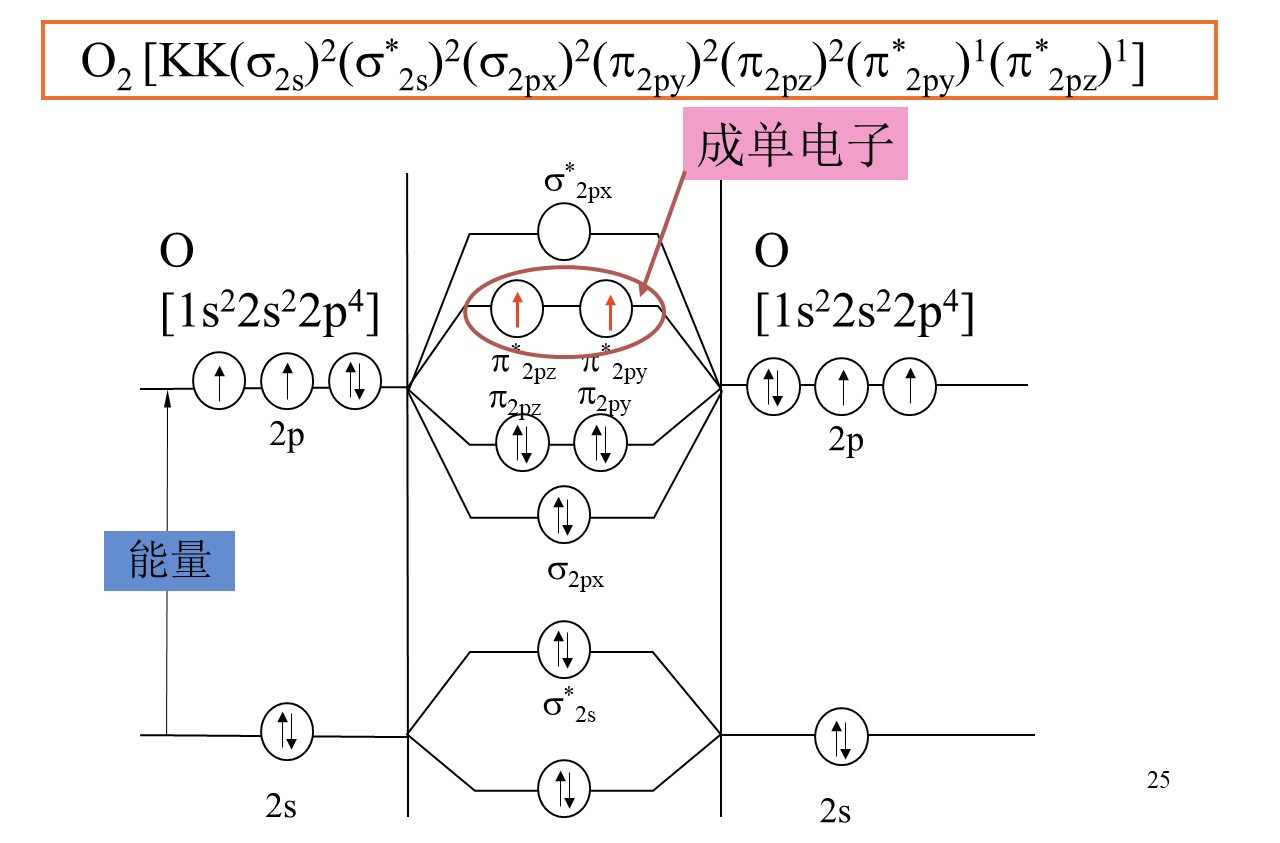
\includegraphics[width=11cm,height=6cm]{oxygen.jpg}
\caption{分子轨道排布}
\end{figure}
%氧为什么没有氮气稳定?
氧形成三电子键,不如氮气的稳定\\
\subsection{金属键}
\subsubsection{金属晶格}
\subsubsection{金属键——改性共价理论}
核对价电子吸引力小,金属的价电子自由脱落,电子在整个金属内自由流动。\\
多个原子共用这些流动的电子,靠这些电子将原子约束在一起\\
金属键的海洋模型: 金属键没有方向性和饱和性\\
金属的特性解释:\\
1. 不透明,金属光泽:吸收许多波长的光线,再次发射出去。\\
2. 导电性:自由电子在外电场下自由流动\\
3. 导热性:自由电子与金属离子碰撞交换能量\\
4. 延展性:正离子间滑动不会导致键的断裂\\
5. 高沸点和气化热:金属不容易摆脱离域负电荷的束缚。
\subsection{分子的极性和分子间力}
对物体的物理性质影响较大
\subsubsection{分子的极性}
{\bf 1. 分子的极性}\\
正负电荷中心不重合,这样的分子就有极性\\
影响因素:分子中化学键、分子的组成和几何构型\\
共价键极性:取决于成键的两个原子的电负性是否相等。
\begin{itemize}
\item 单质中原子电负性相同,故为非极性键
\item 不同原子形成的共价键电子偏向电负性大的一侧,存在极性
\item 双原子分子极性取决于键的极性
\item 多原子分子的极性取决于分子的组成和几何构型(同核:$S_8$;异核:$HX,CO$)
	\subitem 空间构型完全对称,则非极性(根据VSEPR分析)
	\subitem 分子空间构型不对称,极性分子
\end{itemize}
{\bf 2. 分子的偶极矩$\mu$}\\
偶极矩的计算公式
\begin{equation}
\mu = q \cdot d
\end{equation}
偶极矩为矢量,单位$C\cdot m$,方向从负到正\\
{\bf 3. 分子的变型性}\\
将非极性分子置于电场中时,正负电荷中心分离,分子出现偶极,称为诱导偶极。分子越大,变形性越大。\\
{\bf 分子的极化率}\\
诱导偶极的大小与外加电场强度成正比
\[\mu = \alpha E\]
$\alpha$为比例常数。\\
外电场的作用下极性分子顺着电场整齐的排列,这一过程叫做分子的定向极化。\\
极性分子与极性分子、极性分子与非极性分子之间产生微电场,诱导产生偶极\\
瞬时偶极:分子中电子和原子核在运动过程中正负电荷瞬间不重合而产生。\\
\subsubsection{分子间力}
{\bf 1. 取向力}:极性分子固有偶极产生的相互作用力\\
分子极性越大,取向力越大;与绝对温度成反比\\
{\bf 2. 诱导力}\\
极性分子与非极性分子充分接近时,在固有偶极的作用下产生诱导偶极,从而产生作用力。\\
与极性分子的极性正相关,与非极性分子的变形性成正比\\
{\bf 3. 色散力}\\
瞬时偶极之间的相互作用。\\
决定于分子的变形性
{\bf 分子间力的特点}\\
分子间力较弱,比化学键小1~2个数量级\\
分子间作用力是静电引力,没有方向性和饱和性,与分子间距离六次方成反比。\\
色散力$\gg$其余作用力,是最主要的作用力,取向力只有在大分子中才有较大的比重。\\
\subsection{离子极化}
在离子电场的作用下,使周围带异号电荷的离子的电子云发生变形现象。极化力增大导致分子性增强\\
取决于离子的极化力和变形性\\
极化力:
\begin{enumerate}[(1)]
\item 离子半径越小,极化力越大
\item 离子电荷越高,极化力越大
\item 电子构型:18电子,18+2电子>9$\sim$17电子>8电子
\end{enumerate}
变形性:
\begin{enumerate}[(1)]
\item 离子半径 半径越大,变形性越大
\item 负离子离子电荷越高,变形性越大;正离子电荷越高,变形性越小
\item 电子构型:18电子,9$\sim$17电子构型>8电子构型
\end{enumerate}
一般正离子半径小,所以极化力大,变形性小;负离子相反。通常是正离子极化负离子,如果正离子也有一定的变形性(半径较大18电子构型)则也可被负离子极化,极化后的正离子又加强对负离子的极化作用,这称为附加极化。随着极化作用的增强,离子键向共价键过渡。\\
离子极化影响离子的性质:
\begin{enumerate}[(1)]
\item 熔沸点:极化越强,分子性越强,熔沸点越低($Al^{3+}>Mg^{2+}>Na^+$)
\item 溶解度:极化越强,分子性越强,溶解度越低($AgF,AgCl,AgBr,AgI$)
\item 颜色
\end{enumerate}

\newpage
\section{配位化合物}
\subsection{配位解离平衡}
\subsubsection{配位解离平衡和平衡常数}
配位解离平衡在溶液中普遍存在:实质上是配体和水合离子时间的竞争反应。\\
稳定常数K:
\[
K_\text{稳} = \dfrac{[ML_n]}{[M][L]^n}
\]
\[
K_\text{不稳} = \dfrac{[M][L]^n}{[ML_n]}
\]
{\bf 多级配合物的浓度分布特点}\\
各级成分占有一定比例,但是最主要的是最高配位数的配离子。\\
\subsubsection{配位解离平衡的移动}
{\bf 配位平衡和酸碱平衡共存}\\
{\bf 配位平衡和氧化还原平衡}\\
{\bf 配位物之间的转化平衡}\\
由一种配合物转化为另一种更稳定的配合物。\\
\subsection{螯合物的稳定性}

\newpage
\section{元素部分}
\begin{center}
	{\kaishu 只对吉岩老师所画重点进行了总结}
\end{center}
\subsection{s区元素}
\subsubsection{Li,Be的特殊性}
\begin{enumerate}[(1)]
\item 原子半径和离子半径分别是最小的,尤其是$Be^{2+}$共价性超过离子性。
\item 水合能:由于$M^{2+}$有较高的水合能,所以水合能可以抵消第二电离能,故$M^{2+}$稳定存在。
\item $Li$比$Na$更容易失去电子,由于$Li^{+}$拥有较大的水合能。
\end{enumerate}
\subsubsection{元素单质的特殊性}
$Li$燃烧生成氧化物,$Na$生成过氧化物,$K,Rb.Cs$生成超氧化物(大阳离子稳定大阴离子)\\
在与水反应时:$Li$的反应不如和钠反应剧烈,由于生成的$LiOH$溶解度小,阻碍反应进行。\\
氧化物的反应:
\begin{align*}
10Na + 2NaNO_3 = 6Na_2O + N_2\\
CaCO_3 = CaO + CO_2\\
2Na_2O_2 + 2CO_2 = 2Na_2CO_3 + O_2\\
\end{align*}
可以使用离子势来判断金属氢氧化物的碱性
\[\phi = \frac{z}{r}\]
如果$\phi$大,则容易进行酸式解离\\
含氧酸盐的热稳定性:随着半径的减小热稳定性下降(离子极化作用)。碱金属的稳定性高于碱土金属\\
特殊对角线法则:与右下角元素性质接近,如$Li$和$Mg$。因为离子的极化能力接近\\
\subsection{p区元素}
\subsubsection{F的反常性}
$F-F$的键能比$Cl-Cl$小(氟的半径小,孤对电子之间存在斥力),同时$F$的电子亲和能也要比氯小(半径小,电子密度大);\\
从HF到HI:键能下降,稳定性下降;熔沸点,酸性,还原型升高\\
\subsubsection{氯的含氧酸盐}
从氯的氧化数:氧化型下降,酸性升高,稳定性升高\\
\subsubsection{氧族元素}
\begin{enumerate}[(1)]
\item 氧族元素成键规律:如果形成双键的焓变小于二倍的形成单键的焓变,则更容易形成单键;反之容易形成双键;
\item 硫更容易形成单键,单质形式为$S_8$
\item 原因:氧的半径较小,孤对电子之间的斥力导致单键不稳定,但是原子轨道的侧向重叠加大,容易形成多键。
\end{enumerate}
臭氧形成特殊的$\pi^3_4$结构\\
含氧酸盐的极性:随着中心原子的电负性增加酸性增加\\
\subsubsection{氮族元素}
惰性电子对效应:6s电子具有较强的钻穿效应,导致其能量较低,不容易发生反应\\
N和P的区别:氮原子半径较小,容易形成多键的单质;P原子容易形成四面体结构,P-P键能很小\\
\subsubsection{碳族元素}
同样具有惰性电子对效应\\
碳酸盐\\
溶解性:正盐:只有碱金属(除li)和铵的碳酸盐易溶于水;大多数酸式盐易溶于水\\
热稳定性:碳酸盐的热稳定性差,离子极化力越强,分解温度越低\\
\subsubsection{硼族元素}
缺电子化合物:有三个轨道但是只有三个原子,导致容易形成配合物,容易形成聚合分子。\\
硼:$B_2H_6$进行$sp^3$杂化,形成氢桥键\\
硼酸是一元弱酸,只有一级解离\\
\subsection{ds区元素}
ds区元素包括IB和IIB元素,其有效核电荷比s区大,ds区元素的原子半径比s区小得多,电离能也高得多,所以化学性质不甚活泼\\
\subsection{d区元素和f区元素}
特点:属于过渡元素\\
价层电子结构$(n-1)d^{1\sim8}ns^{1\sim2}$\\
单质的相似性:d区元素的最外层电子一般不超过两个,较小的原子半径,较大的密度,较高的熔沸点和良好的导电,导热性\\
可变的氧化态:d电子也可以成键\\
水合离子大多有颜色:分裂能较小,d轨道有未成对电子的元素一般有颜色\\
镧系收缩:镧系元素4f电子的增加不能完全抵消核电荷数的递增,导致镧系元素的半径依次减小,导致镧系收缩\\
\newpage
\section{定量分析的误差和分析结果的数据处理}
\subsection{有效数字}
\subsubsection{有效数字的记位规则}
有效数字就是实际测量能够得到的数字\\
除了最后一位可疑数字之外,其余数字必须是确定无疑的\\
有效数字反映了测量放大的精确度不能随意增减\\
{\bf 1. 有效数字的位数的确定}\\
小数点前和非零数字前的“0”只起定位作用\\
整数末尾的0无法确定其意义\\
在对数值中只有小数点以后的数字计入有效数字\\
改变点位不改变有效数字\\
{\bf 2. 有效数字的修约规则}\\
合理的保留有效数字规则:\emph{”四舍六入五成双“}\\
\subsubsection{有效数字运算法则——先修约后计算}
{\bf 1. 加减法}\\
运算结果绝对误差必须与所有参与运算的数字钟绝对误差最大的数字保持一致,即小数点位数最少的数据为依据。\\
\[32.2 + 20.01 + 0.015 \Rightarrow 32.2 + 20.0 + 0.0 = 52.2\]
{\bf 2. 乘除法}\\
所得结果的有效数字的位数取决于相对误差最大的那个数字\\
\[32.2 \times 20.01 \times 0.015\]
计算可以得到,相对误差最大的数字是0.015,故对所有数据保留两位有效数字
\[32\times 20\times 0.015 = 9.6\]
{\bf 非测量值看做无限位有效数字}\\
e.g.
\[51.996 \times 2 = 103.99 \text{有效数字位数不变}\]
{\bf 4. 分析化学计算习惯}\\
\begin{itemize}
\item 平衡常数保留两到三位有效数字
\item 误差保留一位有效数字,最多两位
\item 对数计算有效数字只计算小数点后的位数
\end{itemize}

\subsection{误差的产生以及表示方法}
\subsubsection{误差产生的原因}
{\bf 1. 系统误差}\\
测定过程中某些始终存在的因素所引起的。具有:\emph{单向性;重现性;可测性;不可通过测量次数消除}\\
分类:
\begin{itemize}
\item 方法误差
\item 仪器和试剂误差
\item 操作误差
\item 环境误差
\end{itemize}
{\bf 2. 随机误差}\\
在测定过程中由于一些难于控制、无法避免的偶然因素引起的。具有:\emph{大小、方向不定;不能通过校正而使其减小或消除;分布服从统计规律;通过增加测定次数可以减小或消除部分}

\subsubsection{误差的表示方法}
(1) 真实值\\
无法精确测得,可以使用代用值:公认真值;精确的测量值;平均值\\
(2) 准确度\\
绝对误差:单次测定:$E = x_i - x_r$ 多次测定:$E = \bar{x} - x_r$\\
相对误差:$E_r = \dfrac{E}{x_r} \times 100\%$\\
(3) 精密度\\
绝对偏差:$d_i = x_i - \bar{x}$\\
绝对偏差:$d_r = \dfrac{d}{\bar{x}} \times 100\%$\\
平均偏差:$\displaystyle\bar{b} = \sum_{i=1}^n|d_i|/n$
相对平均偏差:$ = \dfrac{\bar{b}}{\bar{x}}\times 100\%$
\subsubsection{实验数据处理}
{\bf 标准偏差}
\[
	S = \sqrt{\frac{\displaystyle\sum_{i=1}^n(x_i - \bar{x})^2}{n-1}}
\]
误差用来衡量准确度,偏差用来衡量精密度\\
\emph{精密度高不一定准确度好,准确度高一定精密度好}

\subsection{有限实验数据的统计处理}
\subsubsection{偶然误差的正态分布}
\[
	f(x) = \frac{1}{\sigma\sqrt{2\pi}}e^{-\frac{(x-\mu)^2}{2\sigma^2}}
\]
$f(x)$概率密度函数,表现了无限次测定中,测量值$x$出现的概率情况\\
$\mu$总体平均值,表明数据集中的趋势\\
$\sigma$总体标准偏差,体现了数据的分散性\\
令:
\[
	z = \pm \frac{x-\mu}{\sigma}
\]
则$f(x)$为$z$的函数(标准正态分布):
\[
	f(x) = \frac{1}{\sigma\sqrt{2\pi}}e^{-\frac{z^2}{2}}
\]
\begin{figure}[H]
\centering
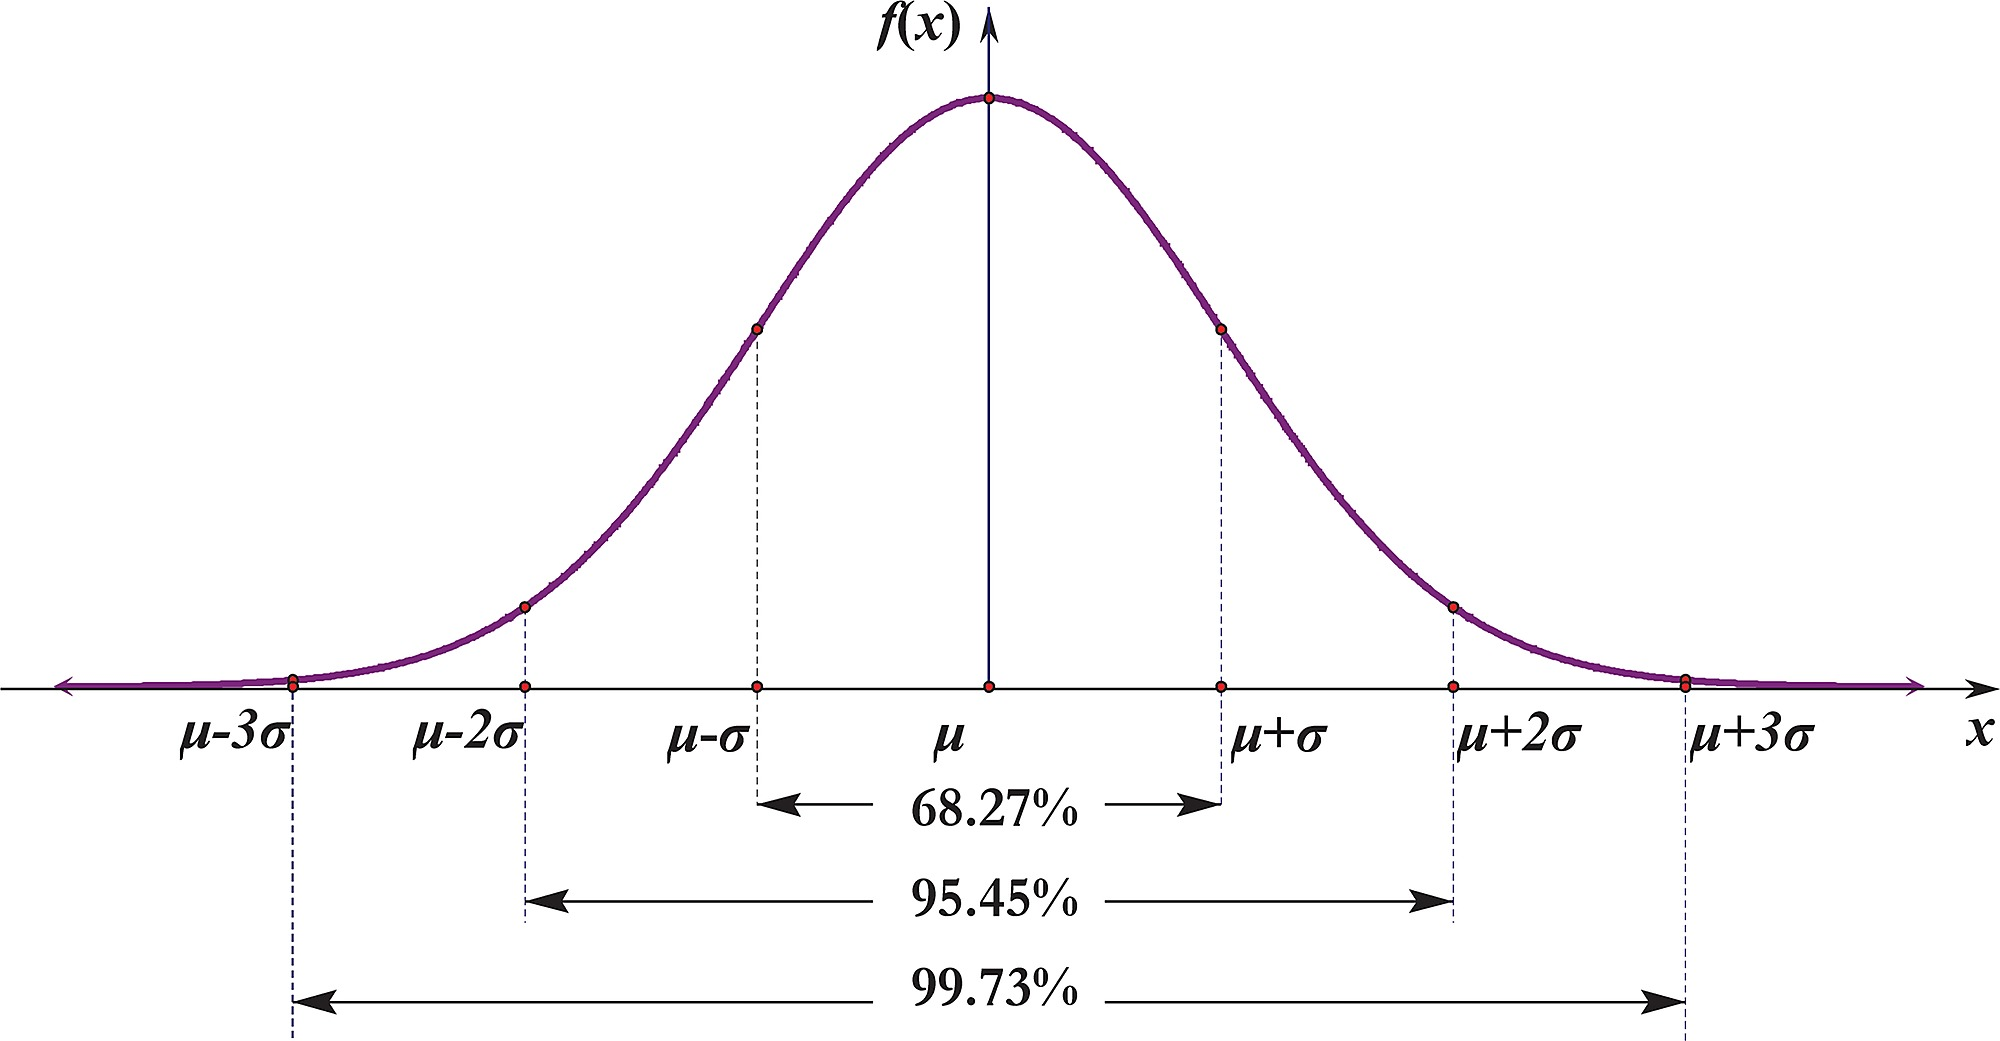
\includegraphics[width = 13cm,height = 7cm]{standard-normal-distribution-curve.jpg}
\caption{正态分布}
\end{figure}
{\bf t分布}\\
在处理少量数据的时候,用$s$代替$\sigma$其分布曲线也发生变化\\
\[
	t = \pm \frac{(\bar{x}-\mu)}{s/\sqrt{n}}
\]
$t$:有限词测量的平均值误差是以平均值的标准偏差为单位表示的数值,这是,偶然误差的分布不服从正态分布。
\[
	\mu = \bar{x}\pm t\frac{s}{\sqrt{n}}
\]
$t$:置信度(查t表)\\
\subsubsection{测定结果离群值舍弃}
\[
	Q = \frac{x_2 - x_1}{x_{max} - x_{min}}
\]
将所有数据按照大小排列,根据测定次数n和置信度查$Q$表,如果$Q$大于临界值,则应该舍弃。\\
\subsubsection{显著性检验}
\subsection{提高准确度的方法}

\section{重量分析方法}
%后期补充
\subsection{影响沉淀纯度的因素}
{\bf 1. 共沉淀}\\
沉淀析出时,在此条件下本来是可溶的杂质也和目标沉淀物一起沉淀下来。\\
吸附共沉淀\\
包藏\\
混晶共沉淀\\
{\bf 2. 后沉淀}\\
沉淀结束后,沉淀和母液放一段时间(陈化),溶液中某些本来难以沉淀的杂质会逐渐析出,而沉淀在被测组分沉淀上。\\
\subsection{沉淀的形成}
沉淀类型:
\begin{table}[H]
\centering
\begin{tabular}{lccc}
\toprule
&晶形沉淀&凝乳状沉淀&无定型沉淀\\
\hline

\end{tabular}

\end{table}
沉淀条件的选择:\\
晶形沉淀:\\
稀溶液中进行,减小过饱和度,生成大颗粒沉淀\\
搅拌,缓慢滴加沉淀剂,避免局部过饱和而生成大量细小晶核\\
热溶液中进行,减小吸附\\
陈化:放置过程中,小晶体溶解,大晶体长得更大\\
非晶形沉淀:\\
在浓溶液中沉淀,减小胶体吸水量,沉淀体积小\\
在溶液中加入挥发性电解质,防止胶溶\\
在热溶液进行\\
不必陈化,沉淀结束后立即过滤,用热水洗涤吸附的杂质。\\
有机沉淀剂的优点:\\
\subsection{重量分析法操作步骤}
{\bf 1. 重量分析法操作步骤}\\
样品溶液制备\\
沉淀制备\\
沉淀过滤,洗涤\\
沉淀烘干或灼烧\\
冷却,称重\\
分析结果计算\\
{\bf 2. 换算因子}\\

\subsection{沉淀的完全程度与影响沉淀溶解度的因素}
\subsubsection{酸效应对沉淀溶解度的影响}
酸效应系数:
\[\alpha = \frac{[A^-] + [HA]}{[A^-]} = \frac{[H^+] + K_a}{K_a}\]
\[[A^-] = \frac{c_0}{\alpha_{A^-(H)}}\]
\[K_{sp} = \frac{s^2}{\alpha_{A^-(H)}}\]
\[s = \sqrt{K_{sp}\cdot\alpha_{A^-(H)}}\]
也可以使用分布系数计算:
\[\alpha_{A^-(H)} = \frac{1}{\delta_{A^-(H)}}\]
\subsubsection{配位效应对沉淀溶解度的影响}
以$AgCl$为例($Cl^-$对于$Ag^+$有配位效应):
\[K_{sp} = \frac{s}{\alpha_{Ag^+}}[Cl^-]\]

\newpage
\section{滴定分析法}
\subsection{滴定分析概论}
\subsubsection{滴定分析过程和方法分类}
滴定分析法:\\
将一种已知浓度的试剂溶液,用滴定管滴加到含有待测组分的溶液中,直到化学反应完成为止。依据试剂与待测组分之间的化学计量关系,计算待测组分含量。\\
\emph{化学计量点:滴定剂的物质的量与被滴定物的物质的量正好符合滴定反应式中的化学计量关系时。\\
滴定终点:指示剂颜色突变而停止滴定的那一点。
}

滴定方法的基本依据:\\
待测组分和所加的化学试剂能发生具有确定计量关系的化学反应。\\
反应能够定量进行到底\\
反应速度快\\
有合适的方法确定反应终点。\\
1. 直接滴定法\\
2. 返滴定法:先计入过量的已知浓度的滴定剂,之后再滴定剩余的滴定剂。\\
3. 置换滴定法\\
4. 间接滴定法\\
\subsubsection{标准溶液的配置、基准物、基准溶液}
标准溶液:已经知道准确浓度的溶液\\
直接法:直接通过基准物进行配置。\\
\emph{基准物:纯度高,组成与化学式相同,性质稳定,有较大的摩尔质量}\\
间接法:先粗配为近似的所需浓度的溶液,然后用基准物通过滴定的方法确定\\

\subsection{酸碱滴定法}
\subsubsection{弱酸弱碱溶液中各物种分布}
分布系数$\delta$(分布分数,摩尔分数)\\
\[
	\delta_A = \frac{A\text{的平衡浓度}}{A\text{各物种总浓度}} = \frac{[A]}{c(A)}
\]
弱酸(碱)水溶液中往往同时存在多种解离形态(物种)。\\
(1) 一元弱酸的分布系数
\begin{align*}
\delta_{HA} = \frac{[HA]}{c} &= \frac{[H^+]}{[H^+]+K_a}\\
\delta_{A^-} &= \frac{K_a}{[H^+]+K_a}
\end{align*}
1. 某酸碱物质组分的分布系数,取决于该酸碱物质的各$K_a$和溶液中的氢离子浓度,可以控制pH来控制某型体的浓度。\\
(2) 多元弱酸的分布系数\\
关于二元弱酸,注意图中所对应的各物种浓度与pH的关系\\
\begin{figure}[H]
\centering
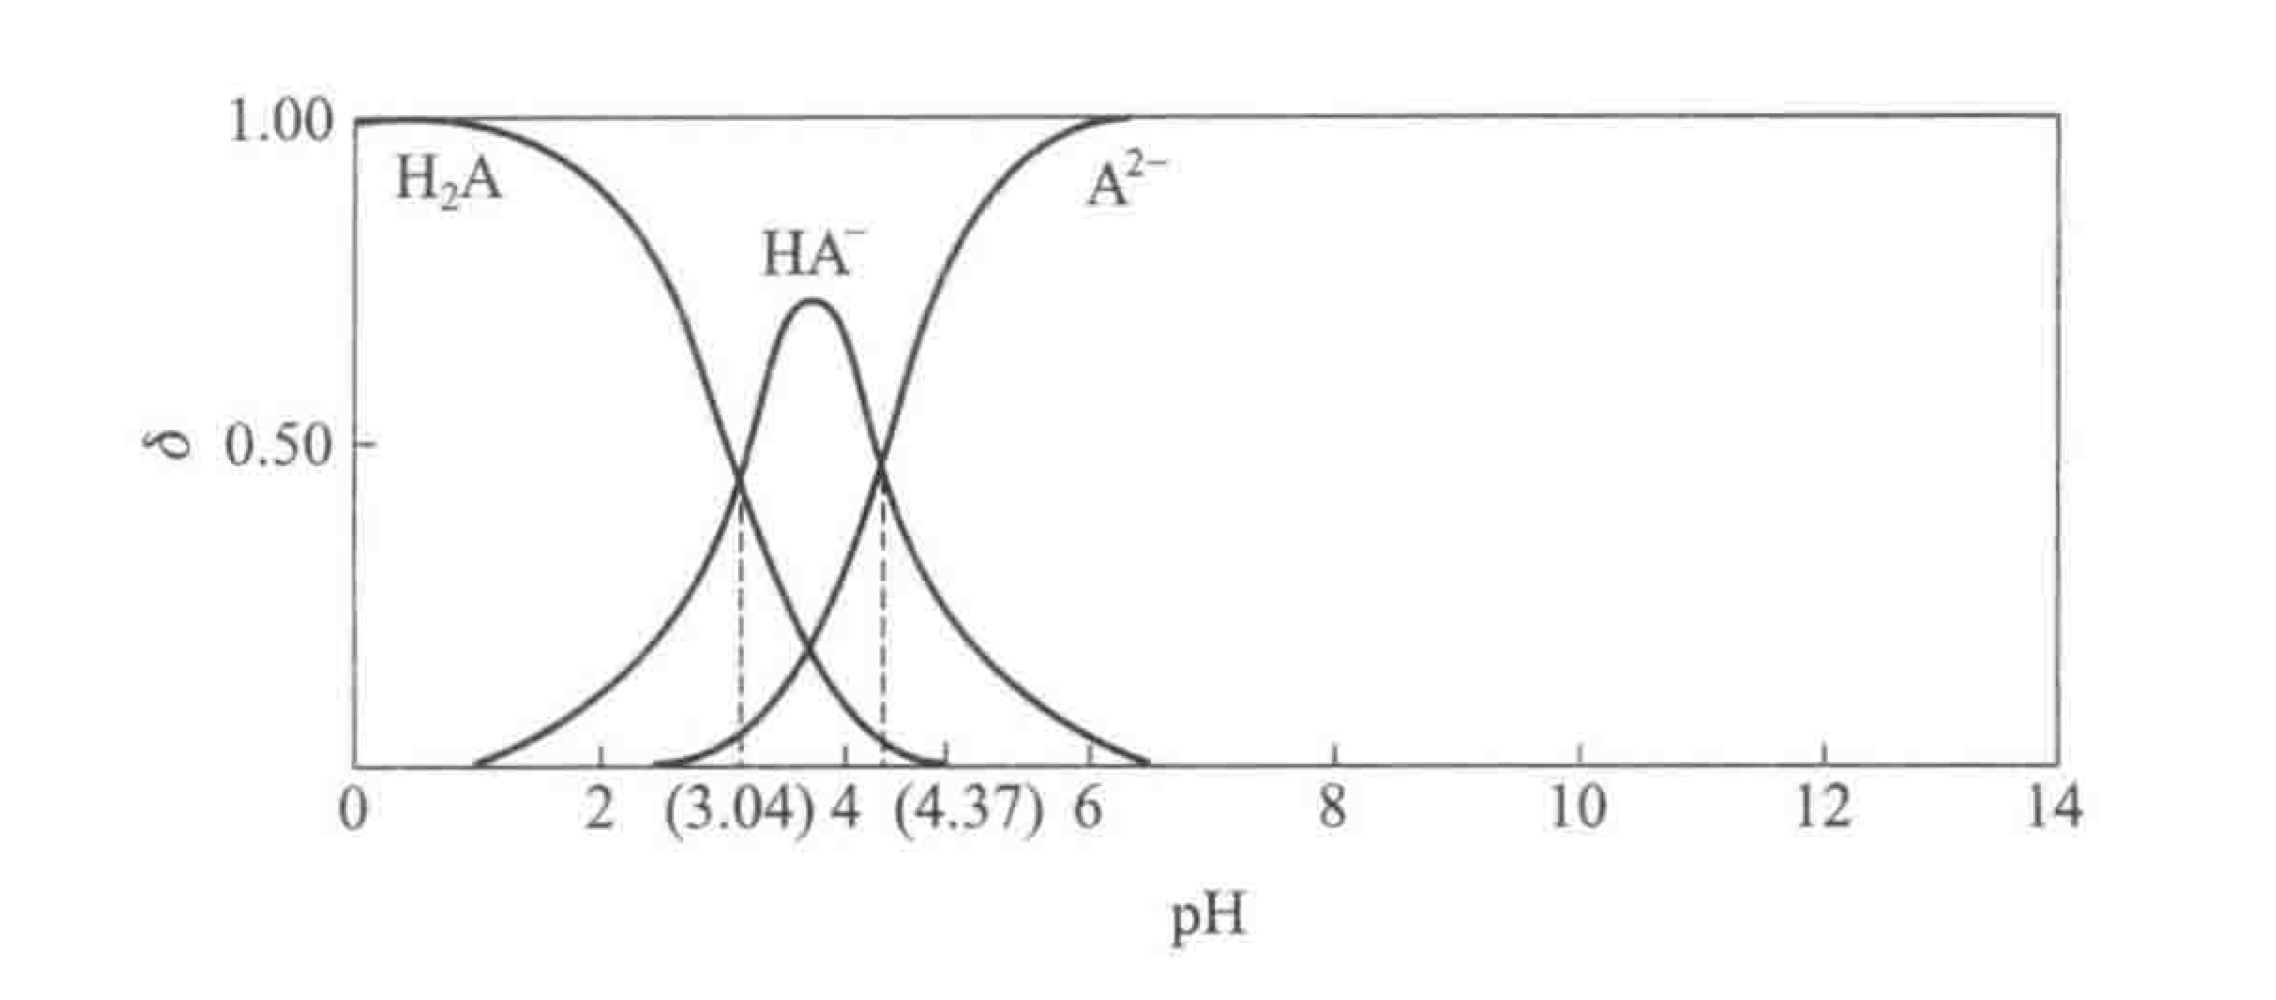
\includegraphics[width = 10cm,height = 5cm]{titration1.jpeg}
\caption{酒石酸曲线图}
\end{figure}
\subsubsection{酸碱溶液中氢离子浓度}
\begin{itemize}
\item 物料平衡
\item 电荷平衡
\item 质子平衡
\end{itemize}
质子条件(平衡)式(PBE)(零水准法)
依据:反应达到平衡时,得质子产物所得质子的数目等于失质子产物所失质子的数目。\\
零水准物质的选择:溶液中大量存在,参与质子转移反应\\
质子条件式书写方法:\\
等式左边——得质子后产物\\
等式右边——失质子后产物\\
1. 一元强酸(强碱)\\
\[PBE: [H^+] = [OH^-] + c\]
c为强酸(强碱)浓度\\
当强酸浓度不是很小$c^2>20k_w$\\
\[[H^+] \approx c\]
当$c$极稀($c^2\leq 20K_w$)\\
\[[H^+] = \frac{K_w}{[H^+]+c}\quad \text{精确式}\]
强碱同理\\
2. 一元弱酸(弱碱)溶液\\
\begin{align*}
[H^+] &= \sqrt{K_a[HA]+K_w}\quad \text{精确公式}\\
c\cdot K_a \geq 20K_w\quad [H^+] &= \sqrt{K_a[HA]}\\
c/K_a \geq 380 \quad[H^+] &= \sqrt{K_ac_0}
\end{align*}
近似公式的展开:
\[[H^+] = \sqrt{K_a(c-[H^+])}\]
\emph{在计算时必须进行充分的分析之后再决定公式的选择}\\
3. 两性物质溶液\\
\begin{align*}
[H^+] &= \sqrt{\frac{K_{a_2}\cdot[HA^-]+K_w}{1+[HA^-]/K_{a_1}}}\\
[H^+] &= \sqrt{K_{a_1}K_{a_2}}
\end{align*} 
\subsubsection{酸碱指示剂}
酸式结构与碱式结构颜色有显著差异的两性物质\\
e.g.\\
{\kaishu
甲基橙:酸色:红色;碱色:黄色\\
酚酞:酸色:无色;碱色:红色\\}
指示剂的变色范围:$pH = pKHln \pm 1$\\
\begin{table}[H]
\centering
\begin{tabular}{lccc}
$[ln^-]/[Hln]:$& >10 & 10$\sim$1/10 & <10\\
溶液中的颜色:& 碱色 & 混合色 & 酸色
\end{tabular}
\end{table}
影响指示剂变色范围的因素:\\
1. 宜少不宜多,看清即可,浓度越大,变色点pH越小\\
2. 温度影响$pK_a$,影响变色间隔\\
3. 溶液离子强度:影响$pK_a$\\
4. 溶剂\\
混合指示剂:利用颜色的互补作用,使颜色变化更加敏锐,和变色范围更窄\\
\subsubsection{酸碱滴定的滴定曲线及指示剂的选择}
滴定曲线:\\
滴定pH随滴定剂加入量或滴定分数T变化的曲线\\
{\bf 1. 强碱滴定强酸}\\
滴定过程中pH变化规律:\\
a. 滴定前:\\
$[H^+] = c_0 = 0.1000mol/L$\\
b. 滴定开始后,到化学计量点之前\\
$[H^+] = \dfrac{n_{H^+}}{V} = \dfrac{c_0(V_0 - V)}{V + V_0}$\\
假定滴加的氢氧化钠体积为$19.98ml$  pH = 4.30\\
c. 化学计量点\\
此时,pH = 7\\
d. 化学计量点之后\\
超过0.02ml时,pH = 9.70\\
突跃范围:浓度越大,范围越大\\
\emph{根据突跃范围选择合适的指示剂}\\
{\bf 2. 强碱滴定一元弱酸}\\
a. 滴定前:\\
$[H^+] = \sqrt{c_0K_a}$\\
b. 滴定开始后,到化学计量点之前\\
$pH = pK_a + \lg\frac{[Ac^-]}{HAc}$\\
c. 化学计量点\\
$[OH^-] = \sqrt{K_{b(Ac^-)}\cdot c_{Ac^-}}$\\
d. 化学计量点之后\\

一元弱酸可以被强碱准确滴定的判据:\\
必须要有足够大的突跃范围,保证可以判断滴定终点\\
影响突跃范围的两个因素:一元弱酸的强度和浓度\\
人眼对于指示剂变色的盘点至少存在$\pm 0.2$的误差\\
\subsubsection{酸碱滴定法的应用}
混合碱的分别滴定(双指示剂法)\\
$NaOH + NaCO_3$\\

\subsection{配位滴定法}
\subsubsection{配位滴定法概述}
基于配位反应的滴定分析法\\
无机配体:稳定性不高,不能满足滴定需求\\
有机配体:适合用来滴定\\
最广泛的滴定配体:EDTA二钠\\
特点:普遍性,稳定性,配合比简单(1:1),亲水性,颜色\\
{\bf 副反应}
\begin{figure}[H]
\centering
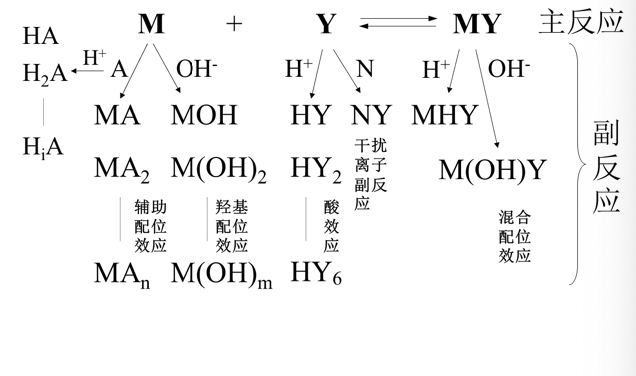
\includegraphics[width=14cm, height=10cm]{side reaction.png}
\caption{副反应类型}
\end{figure}
存在副反应时,定量表示副反应程度,引入副反应系数$\alpha$
\[\alpha_M = \frac{[M']}{[M]}\quad \alpha_Y = \frac{[Y']}{[Y]}\quad\alpha_{MY} = \frac{[MY']}{[MY]}\]
1) 滴定剂Y副反应系数\\
副反应系数表示:未与M配位的滴定剂的各物种的总浓度是游离滴定剂平衡浓度的多少倍,当没有副反应时,$\alpha_Y = 1$\\
\emph{酸效应:溶液中$H^+$与Y发生副反应使得EDTA配位能力下降,使用酸效应系数$\alpha_{Y(H)}$表示}
\[\alpha_{Y(H)} = 1 + \sum^6_{i=1}\beta^H_i[H^+]^i\]

2) 金属离子M副反应系数\\
在pH较大的溶液中容易出现金属离子水解产生羟基配合物,掩蔽剂也可能与待测离子形成配合物。\\
3) MY副反应可以忽略不计\\
条件稳定常数:
\[K'_{MY}\frac{[MY']}{[M'][Y']} = \frac{\alpha_{MY}}{\alpha_M\alpha_Y}K_{MY}\]
通常MY副反应系数可以忽略不计
\[\lg K'_{MY} = \lg K_{MY} - \lg\alpha_M-\lg\alpha_Y\]
副反应存在的条件下,在具体的实验条件下,条件稳定常数越大,主反应进行的越完全。\\

\subsubsection{配位滴定基本原理}
{\bf 1. 配位滴定曲线}\\
\[[M']\text{(化学计量点)} = \sqrt{\frac{c(M,\text{化学计量点})}{K'_{MY}}}\]
\[p[M'] = \frac{1}{2}(pK'_{MY} - pc)\]
影响滴定突跃的因素:条件稳定常数(一定条件下与突跃正相关),被测金属离子浓度\\
降低溶液酸度可以提升$K'_{MY}$从而加大滴定突跃。\\
被测金属浓度越大滴定突跃越大\\
{\bf 2. 滴定指示剂}\\
使用金属指示剂指示终点\\
主要条件:\\
1) 配合物颜色和指示剂颜色有明显区别\\
2) MIn稳定性低于M-EDTA稳定性,否则EDTA不能夺取M,称为\emph{指示剂的封闭}\\
3) 指示剂与金属离子反应迅速、灵敏、迅速,具有良好的变色可逆性。若指示剂溶解度过低,会导致交换反应缓慢,终点延长,称为\emph{指示剂的僵化}\\
4) 指示剂应该比较稳定\\
{\bf 3. 指示剂酸度选择}\\
通过酸效应曲线判断,考虑金属的水解和指示剂的选择\\
\subsubsection{混合离子滴定}
{\bf 1. 酸度控制法}\\
最高酸度\\
\[\lg\alpha_{Y(H)}\leq \lg K + \lg c - 6\]
当$c = 0.01 mol/L$
\[\lg\alpha_{Y(H)}\leq \lg K - 8\]
最低酸度: 金属离子开始产生沉淀时的pH\\
\[[OH^{-}] = \sqrt{\frac{K_{sp}}{[M]}}\]
在进行滴定时,若两金属离子在酸度条件下,其中一种离子可以准确滴定,另一种不能。\\
{\bf 2. 用掩蔽的方法进行滴定}\\
1) 配位掩蔽法:使用能与干扰离子形成稳定配合物的配位基\\
2) 氧化还原掩蔽法:改变干扰离子的氧化数\\
3) 沉淀掩蔽法\\
对于掩蔽剂的要求:\\
1) 掩蔽剂与干扰离子结合能力比EDTA强\\
2) 掩蔽剂不与待测离子配位或者配位的倾向很小\\
3) 生成的配合物应该是无色的或浅色的\\
4) pH范围与所使用的的pH范围一致
\subsubsection{配位滴定的方式和应用实例}
(1) 直接滴定法\\
(2) 返滴定法:加入过量EDTA,再使用金属离子滴定剩余的EDTA(如滴定$Al^{3+}$)\\
(3) 置换滴定法

\subsection{氧化还原滴定}
\subsubsection{概述}
{\bf 氧化还原反应能否滴定的判据}\\
条件电极电势:\\
考虑氧化态物质和还原态物质的活度系数($\gamma$)和副反应系数($\alpha$)\\
\[\phi^{\theta'} = \phi^{\theta} + \frac{0.0592}{n}\lg\frac{\alpha_{Red}\gamma_{Ox}}{\alpha_{Ox}\gamma_{Red}}\]
{\bf 反应速度问题}\\
反应分布进行:\\
影响速度的因素:反应物浓度,温度,催化剂

\subsubsection{氧化还原滴定法基本原理}
{\bf 滴定曲线}
\[Ce^{4+} + Fe^{2+} = Ce^{3+} + Fe^{3+}\]
a. 滴定开始之前($Fe^{2+}$无法计算)\\
b. 滴定开始到化学计量点之前\\
根据滴定剂的消耗量可以求出溶液中剩余的亚铁离子和生成的铁离子。于是可以求铁电位求体系电位。
\[\phi = \phi^{\theta'} + 0.0592\lg\frac{V}{V_0 - V}\]
c. 化学计量点\\
不能用单一电对计算体系电位值,需要联系两个能斯特方程。
\[\phi_{\text{计}} = \frac{z_1\phi_1 + z_2\phi_2}{z_1 + z_2}\]
突跃范围:
\[\phi_{\text{计}} + \frac{3\times 0.0592V}{z_2} \sim\phi_{\text{计}} - \frac{3\times 0.0592V}{z_1} \]
滴定突跃范围
d. 化学计量点之后\\
滴定突跃:突跃大小决定于两电对的条件电极电势差。\\
{\bf 终点指示方法}\\
1) 自身指示剂\\
2) 特殊指示剂,如淀粉与碘\\
3) 氧化还原指示剂,随着环境氧化还原电位的变化改变颜色\\
变色范围:
\[\phi_{In}^{\theta'} \pm \frac{0.0592V}{z}\]
\subsubsection{氧化还原预处理}
预处理要求:反应速度快,能将组分还原或氧化,选择性好,过量的氧化还原剂容易除去\\
\subsubsection{氧化还原滴定法}
一般用氧化剂作为滴定剂,如果用还原剂要防止被空气中的氧氧化\\
氧化还原滴定法类型\\
1. 高锰酸钾法(自身指示剂)\\
\quad 氧化能力强,间接测定多种无机物和有机物,本身可以作为指示剂\\
\quad 标准溶液不够稳定,滴定选择性差\\
标定:草酸还原\\
滴定条件
\begin{itemize}
\item 温度:70-80度
\item 酸度:$1mol/L^{-1}H_2SO_4$(不可以使用盐酸)
\item 滴定速度:慢(否则$KMnO_4$来不及反应分解) - 快 - 慢
\end{itemize}
应用:直接滴定、间接滴定(草酸根与金属产生沉淀,滴定草酸根)、返滴定($MnO_2$与有机物)\\
2. 重铬酸钾法\\
特点:纯、稳定、直接配置标准溶液、可以使用$HCl$作为介质\\
3. 碘量法\\
大pH范围内不受酸度影响\\
淀粉与碘变色灵敏\\
误差:$I_2$易挥发\\
应用:测定维生素C、铜、葡萄糖\\
4. 溴酸钾法\\

\subsection{沉淀滴定法}
主要以银的难溶盐沉淀反应为基础的银量法\\
突跃范围:难溶盐溶解度越小,突跃范围越大;浓度越大,突跃范围越大。\\
\subsubsection{莫尔(Mohr)法}
1. 方法原理:在中性或弱碱性溶液中,以铬酸钾为指示剂,用$AgNO_3$标准溶液直接滴定$Cl^-$\\
2. 终点指示:$Ag_2CrO_4$的溶解度大于$AgCl$,所以达到终点时生成砖红色沉淀\\
3. 指示剂用量:过大则终点早出现,过小则终点晚出现
\[[CrO_4^{2-}] = \frac{K_{sp(Ag_2CrO_4)}}{K_{sp(AgCl)}} = 0.006mol/L\]
4. 实验条件:中性或弱碱性
5. 局限性:只能测氯离子和溴离子,不能用$NaCl$滴定,干扰较多
\subsubsection{佛尔哈德法}
1. 方法原理:强酸性溶液中用铁铵矾作为指示剂,以$NH_4SCN$作为标准溶液滴定$Ag^+$\\
2. 终点指示:化学计量点附近,过量$SCN^-$与$Fe^{3+}$生成红色的配合物\\
3. 滴定方法:直接滴定测$Ag^-$、返滴定\\
\subsubsection{法扬司法}
使用吸附指示剂指示终点\\
在化学计量点之前,$Cl^-$过量,荧光黄阴离子难以吸附在沉淀上,溶液为黄绿色\\
达到化学计量点之后,过量的$Ag^+$使沉淀吸附层带正电荷,溶液中的荧光黄阴离子被带正电荷的胶状沉淀吸附,因吸附而发生分子结构的变化,从而引起颜色变化(黄绿色变为粉红色)\\

\newpage

\section{比色法与分光光度法}
\subsection{概述}
\subsubsection{分光光度法及其特点}
\subsection{光吸收定律}
朗伯-比尔定律:
\[A = \lg\frac{I_0}{I} = kbc\]
当b的单位为cm,c的单位为mol/L,吸光系数为摩尔吸光系数$\epsilon$,单位为$cm^{-1}mol^{-1}L$$\epsilon$越大,检测灵敏度越高(决定波长的选取)\\
适用范围:\\
1)溶液、气态和固态吸光物质\\
2) 各种吸光光度法定量分析的依据\\
注意\\
1)单色光\\
2)吸光质点形式不变\\
3)稀溶液\\
标准曲线\\
测定信号随被测浓度变化\\
在工作曲线过高浓度时导致偏离、曲线不过原点等\\
原因:\\定律本身的局限性:架设了吸光分子之阿没有相互作用\\入射光不是单色光\\
化学因素引起的偏离:\\介质不均匀\\吸光分子发生化学变化\\温度对化学平衡的影响
\subsection{比色法和分光光度法及其仪器}
1. 光度分析方法\\
目视比色法:从样品上方观察\\
光电比色法\\
分光光度计:\\
分光光度计的基本部件:\\
光源:发出所需波长范围内的连续光谱\\
\end{document}